%% Esempio per lo stile supsi
\documentclass[twoside]{template} 

% per settare noindent
\setlength{\parindent}{0pt}


% Crea un capitolo senza numerazione che pero` appare nell'indice %
\newcommand{\problemchapter}[1]{%
  \chapter*{#1}%
  \addcontentsline{toc}{chapter}{#1}%
\markboth{#1}{#1}
}

% Numerazione delle appendici secondo norma
\addto\appendix{
\renewcommand{\thesection}{\Alph{chapter}.\arabic{section}}
\renewcommand{\thesubsection}{\thesection.\arabic{subsection}}}

% Extra packages needed by the Models chapter (tables, diagrams, code/prompt listings)
\usepackage{booktabs}
\usepackage{longtable}
\usepackage{xcolor}
\usepackage{listings}
\usepackage{seqsplit}
\usepackage{tikz}
\usetikzlibrary{positioning,arrows.meta,shapes.geometric,fit}

\lstdefinestyle{jsonstyle}{
  basicstyle=\ttfamily\footnotesize,
  breaklines=true,
  columns=fullflexible,
  frame=single,
  backgroundcolor=\color{black!3},
  showstringspaces=false
}
\lstdefinestyle{promptstyle}{
  basicstyle=\ttfamily\small,
  breaklines=true,
  columns=fullflexible,
  frame=single,
  backgroundcolor=\color{black!3},
  showstringspaces=false
}

\setcounter{secnumdepth}{5} 	%per avere più livelli nei titoli
\setcounter{tocdepth}{5}		%per avere più livelli nell'indice


\titolo{Titolo}
\studente{Student}
\relatore{Supervisor}
\correlatore{Co-supervisor}
\committente{Host(s)}
\corso{Data Science and Artificial Intelligence}
\modulo{Diploma Thesis}
\anno{2025}



\begin{document}

\pagenumbering{alpha}
\maketitle
\onehalfspacing
\frontmatter
\raggedbottom 

\pagenumbering{roman}
\tableofcontents
\listoffigures					% Opzionale
\listoftables					% Opzionale

\newpage
\mainmatter
\pagenumbering{arabic}
\setcounter{page}{1}

\chapter{Introduction}

\section{Background and motivation}

Academic and domain-specific terminology often admits multiple valid lexical formulations for the same underlying concept, and semantic relatedness does not necessarily imply strict synonymy: a term can be topically or associatively close to another without being an acceptable substitute for it. Retrieving the specific synonym intended for a given term from a controlled terminology inventory is therefore a non-trivial ranking problem, distinct from general semantic-similarity search.

This thesis studies that problem empirically, comparing lexical retrieval, dense embedding retrieval, Large Language Model (LLM)-based query expansion, and LLM-based reranking as different mechanisms for identifying the intended synonym of an English academic or domain term, and comparing a fixed-role multi-agent pipeline against a more autonomous, dynamic tool-calling alternative for orchestrating these mechanisms.

\section{Research problem and task formulation}

Given an input academic or domain term, the system ranks candidates from a fixed terminology inventory and is evaluated according to the position of the row-specific annotated synonym. The task is formulated as \textbf{transductive, closed-pool synonym ranking}: a global candidate vocabulary is available in full at evaluation time, including candidate strings associated with validation and test rows, while the correct mapping between an individual input term and a vocabulary entry remains hidden from the system until after a prediction has been produced. This formulation differs from unrestricted synonym generation, since every returned answer must belong to the fixed inventory; the reported results measure ranking and selection quality within that known inventory and should not be interpreted as evidence of the ability to generate synonyms outside it.

The candidate vocabulary is derived from the dataset prepared for the task. One degenerate identity pair -- an input term recorded as its own synonym -- is then removed to form the final evaluation dataset (Chapter~\ref{chap:data}), which contains 969 rows. The candidate vocabulary itself has a verified cardinality of 921 candidate synonyms.

\section{Research objectives}

The project was structured around the following objectives, each evaluated empirically under a common protocol:

\begin{itemize}
  \item evaluate lexical retrieval and dense embedding retrieval as baseline approaches to closed-pool synonym ranking;
  \item evaluate LLM-based query expansion, and deterministic weighted multi-query fusion as a mechanism for controlling its contribution;
  \item evaluate LLM-based reranking of a retrieved shortlist, including its sensitivity to reranker model capability;
  \item compare a fixed-role, centrally orchestrated multi-agent architecture against a dynamic, single-agent tool-calling architecture under matched downstream retrieval and reranking components;
  \item examine the accuracy--latency--cost trade-offs across the resulting configurations.
\end{itemize}

\section{Proposed approach}

The system evaluated as the primary configuration is a \textbf{fixed-role, centrally orchestrated multi-agent pipeline}. A Generator Agent, an LLM-based component, produces query variants and paraphrases of the input term. Deterministic retrieval and weighted fusion -- supporting software components, not agents -- use these variants to score and shortlist candidates from the closed vocabulary using dense embeddings. A Verifier/Reranker Agent, a second LLM-based component, then evaluates and reorders that shortlist to produce the final prediction. Neither retrieval nor fusion negotiates, plans, or allocates tasks; coordination between the two agents is centralized rather than decentralized.

As an alternative, the project also implements and evaluates a \textbf{dynamic tool-calling architecture}, in which a single controller agent decides at runtime, rather than through a fixed expansion strategy, which retrieval queries to issue and how many retrieval calls to perform before finalizing its candidate list. Retrieval remains a tool invoked by this controller, not an agent in its own right. The two architectures are compared experimentally under a matched downstream configuration, sharing the same retrieval model and final reranker (Chapter~\ref{chap:results}).

\section{Thesis structure}

The remainder of this thesis is organized as follows. Chapter~\ref{chap:data} (Data) describes the source dataset and its documented provenance, the construction of the project-specific dataset and closed candidate vocabulary, preprocessing and normalization, the train/validation/test partitioning protocol, and the resulting task and leakage boundaries. Chapter~\ref{chap:models} (Models) presents the baseline model families, the fixed-role multi-agent pipeline and the dynamic tool-calling architecture in detail, the prompts and interface contracts used by each agent, engineering trade-offs across configurations, and the formal evaluation protocol. Chapter~\ref{chap:results} (Results) reports the main quantitative results, validation ablations, the fixed-versus-dynamic architecture comparison, the accuracy--latency trade-off, error analysis, and statistical interpretation of the reported differences. Chapter~\ref{chap:conclusions} (Conclusions) revisits the research objectives in light of the experimental evidence, synthesizes the methodological choices and results, discusses limitations and engineering recommendations, and proposes future work.

\chapter{Data}
\label{chap:data}

\section{Executive summary}

This chapter describes the dataset used to construct and evaluate the closed-pool synonym-ranking system: the origin and documented provenance of the public source; how the project-specific dataset and its closed candidate vocabulary were built; the unit of observation and its single-label limitation; string normalization; the composition of the retained terms; and the grouped train/validation/test partitioning. Data-related limitations are discussed together with the project's other limitations in the Conclusions chapter.

The public source contains 1,266 records. After removing rows with an unusable input term, removing exact duplicate pairs, and removing one identity pair, the project retains 969 rows for evaluation. The closed candidate vocabulary of 921 unique synonym strings is built one step earlier, from the 970-row table that still includes the identity pair, so that the synonym it contributes remains a valid candidate even though the identity row itself is excluded from evaluation. These 969 rows are partitioned, by exact input term and with a fixed random seed (42), into 581 training, 194 validation, and 194 test rows.

\section{Dataset origin and scope}

The source dataset is published on Hugging Face under the identifier \texttt{\seqsplit{jensjorisdecorte/TU-Expert-Collection-Topic-Synonyms}} (Hub revision \texttt{\seqsplit{fb767656de4cb453d3b4d88bcdd060ee17a81f4b}}, last modified 2024-09-23). At this revision, the repository exposes one split, named \texttt{train}, containing 1,266 records with the following fields: an integer row index; a \texttt{topic} identifier such as \texttt{topic-12722}; an English term (\texttt{en}) and its Dutch counterpart (\texttt{nl}); and an English synonym (\texttt{en\_synonym}) with its Dutch counterpart (\texttt{nl\_synonym}).

The repository does not provide detailed documentation on the dataset's original collection or annotation procedure.

The public data is bilingual and covers heterogeneous terminology, including examples from economics, law, psychology, information systems, religion, education, and public policy. Some records have a missing, empty, or placeholder value in the English term field while the English synonym field remains populated; the exact effect of this on the retained dataset is quantified in the next section.

\section{Project-specific dataset construction}

The project retains only the two fields required by the ranking task: \texttt{en}, the input query term, and \texttt{en\_synonym}, the row-specific relevant candidate. The \texttt{topic}, \texttt{nl}, and \texttt{nl\_synonym} fields, and the numeric row index, are not passed to any evaluated method. This restricts the task to English-only synonym ranking and prevents auxiliary fields from influencing candidate generation or ranking.

The reduction from the public source to the final evaluation dataset proceeds in three filtering steps. Of the 1,266 source rows, 284 have an invalid \texttt{en} value (null, empty, or the placeholder ``\texttt{-}'') and are removed. A further 12 rows are exact duplicate (\texttt{en}, \texttt{en\_synonym}) pairs and are removed, leaving a prepared table of 970 rows. Finally, the single identity row in which the input term and its recorded synonym coincide (\emph{modernisation}--\emph{modernisation}) is removed, leaving the 969-row evaluation dataset. This identity row is removed because the retrieval implementation excludes the input term from its own candidate list; for an identity row, that exclusion would leave no correct candidate available.

Each retained row represents one evaluation instance: one input academic or domain term and one row-specific expected English synonym. The dataset is therefore not a conventional multiclass classification dataset with a small set of balanced classes; it is a ranking dataset in which each query has one labeled relevant item within a much larger shared candidate vocabulary.

For a candidate vocabulary of size $V$, each row contains one labelled relevant candidate and $V-1$ candidates treated as non-relevant under the single-label evaluation protocol used for scoring. This is a statement about the evaluation protocol, not a claim that the remaining $V-1$ candidates are necessarily semantically incorrect for that row: a candidate that is not labelled as relevant for a given row is simply not the row's recorded gold value, and may still be a plausible synonym.

This distinction matters because ten input terms occur twice in the evaluation dataset, each time paired with a different recorded synonym. Given 969 rows with ten terms occurring twice, the evaluation dataset contains 959 distinct input strings (the corresponding prepared, 970-row table contains 960 distinct input strings, one more because it still includes the removed identity row).

\section{Candidate vocabulary}
\label{sec:candidate-vocab}

The project adopts a closed-pool ranking formulation, and it is necessary to distinguish two datasets that this formulation depends on. Let the prepared dataset, obtained after removing invalid rows and exact duplicates, be

\[ D_{\mathrm{prepared}} = \{(q_i, y_i)\}_{i=1}^{970}, \]

and let the evaluation dataset, obtained after additionally removing the identity pair, be

\[ D_{\mathrm{eval}} = \{(q_i, y_i)\}_{i=1}^{969} \subset D_{\mathrm{prepared}}, \]

where $q_i$ is an English input term and $y_i$ is its recorded English synonym. The global candidate vocabulary is built from the prepared dataset, \emph{before} the identity pair is removed:

\[ C = \operatorname{unique}\left(\{y_i \mid (q_i,y_i) \in D_{\mathrm{prepared}}\}\right), \qquad |C| = 921. \]

The train, validation, and test partitions (Section~\ref{sec:partitioning}) are derived from $D_{\mathrm{eval}}$, not from $D_{\mathrm{prepared}}$. Consequently, the candidate vocabulary $C$ still contains the synonym string contributed by the excluded identity row, even though that row itself is never scored, since it does not appear in $D_{\mathrm{eval}}$ or in any split derived from it.

The vocabulary is built by deduplicating the retained synonym values under a shared normalization rule, defined in full in Section~\ref{sec:normalization}: each string is lowercased and stripped of surface punctuation before comparison, so that, for example, \emph{IT-Governance} and \emph{it governance} are treated as the same candidate. For each normalized value, the first surface form encountered is the one retained, and entries are kept in the order in which they were first observed rather than sorted alphabetically. Equality among candidates, and between a candidate and a row-specific gold value, is evaluated after this normalization, so entries differing only in case or surface punctuation are not treated as distinct. For every input term, the system produces an ordered list of candidates selected from $C$; the raw output of any language model used for query expansion is not treated as a final answer unless it corresponds to an entry of $C$, so every method, including the ones that free-generate a candidate proposal, ultimately returns a member of the closed vocabulary rather than unconstrained text.

\section{Preprocessing and normalization}
\label{sec:normalization}

\subsection{Stored representation}

The stored dataset retains the original surface form of each string after basic cleaning: leading and trailing whitespace is removed, and empty strings or the placeholder ``\texttt{-}'' are treated as missing values and dropped.

\subsection{Equality representation}

Independently of the stored representation, every equality check performed by the project -- candidate deduplication, exclusion of the input term from its own candidate list, and matching a prediction against the row-specific gold label -- uses a shared normalized form of each string: lowercased, stripped of leading and trailing whitespace, filtered to remove characters outside basic ASCII letters, digits, whitespace, and hyphens, with the remaining whitespace collapsed. This filter deletes unsupported characters rather than transliterating them to an ASCII equivalent, so an accented character is removed rather than folded to its unaccented counterpart; given that the retained fields are English-language academic terminology, this is expected to affect a small share of entries. The stored strings themselves are not modified by this process -- it is used only for equality comparisons.

\section{Dataset composition}

\subsection{Term-type distribution}

The 969-row evaluation dataset is divided into four mutually exhaustive, heuristically defined term types: abbreviation-like terms, compounds, multi-word phrases, and single words. A term is classified as abbreviation-like if it is a single token that is either fully uppercase or at most five characters long; a single token that does not meet this criterion is a single word; among multi-token terms, a term containing a hyphen or consisting of exactly two words is a compound; every remaining multi-token term is a multi-word phrase. These are project-specific analytical categories rather than authoritative linguistic classes, but the classification rule is deterministic, with no ambiguous cases. Table~\ref{tab:term-types} reports the resulting distribution.

\begingroup
\footnotesize
\begin{table}[htbp]
\centering
\begin{tabular}{lrr}
\toprule
\textbf{Term type} & \textbf{Rows} & \textbf{Dataset share}\\
\midrule
Abbreviation-like & 34 & 3.5\%\\
Compound & 432 & 44.6\%\\
Multi-word phrase & 250 & 25.8\%\\
Single word & 253 & 26.1\%\\
\midrule
Total & 969 & 100.0\%\\
\bottomrule
\end{tabular}
\caption{Descriptive term-type distribution of the 969-row evaluation dataset. Model performance broken down by these categories is reported in the Results chapter.}
\label{tab:term-types}
\end{table}
\endgroup

Compounds form the largest category, at approximately 44.6\% of the dataset; multi-word phrases and single words each represent approximately one quarter; abbreviation-like inputs form a comparatively small subset. A lexical-overlap indicator, based on shared whitespace-separated tokens between an input term and its gold synonym, was also defined for post-hoc error analysis; the corresponding performance results are reported in the Results chapter rather than here.

\section{Train, validation, and test partitioning}
\label{sec:partitioning}

The 969-row evaluation dataset was partitioned with a fixed random seed (42) and a nominal 60/20/20 allocation, producing 581 training rows, 194 validation rows, and 194 test rows. The partition is grouped by the exact input term rather than by row, so that every occurrence of a repeated input term is assigned to the same partition. This grouping is necessary because ten input terms occur twice with different recorded synonyms: without it, one occurrence of a term could be used for configuration decisions while another occurrence of the same term, with a different gold label, appeared in the test partition.

Table~\ref{tab:partitions} summarizes each partition's size and its actual role in the project.

\begingroup
\footnotesize
\begin{table}[htbp]
\centering
\begin{tabular}{p{2.2cm}p{1.2cm}p{1.3cm}p{8.6cm}}
\toprule
\textbf{Partition} & \textbf{Rows} & \textbf{Share} & \textbf{Role in this project}\\
\midrule
Train & 581 & 59.96\% & Not used to fit or select any of the reported systems.\\
Validation & 194 & 20.02\% & Used throughout the project for model, fusion, and configuration decisions.\\
Test & 194 & 20.02\% & Not used for direct parameter or model selection; several already-selected configurations were evaluated on it at different points as the experimental process progressed.\\
Full & 969 & 100.00\% & Not an independent split; the union of the three partitions, used only for descriptive reporting and error analysis after a final configuration had been selected.\\
\bottomrule
\end{tabular}
\caption{Role of each partition, as actually used in this project.}
\label{tab:partitions}
\end{table}
\endgroup

The training partition is not used to fit or select any of the evaluated systems: no component in this project is trained with gradient descent, so there is no model-fitting step for it to support. It is reserved, unused, so that a future extension of this project -- for example, fitting fusion weights or a confidence threshold on data the reported comparisons never touched -- would still have a partition available that has not influenced any decision made in this thesis. The validation partition, by contrast, was used throughout the project to choose between embedding models, fusion strategies, query-expansion settings, candidate-pool widths, and rerankers.

The test partition was not used to choose between candidate methods or parameter values -- those decisions were made on the validation partition. It was, however, evaluated more than once: as the pipeline evolved, several configurations already selected on validation were subsequently run on the test partition at different points during the project, and their results are reported alongside the final configuration in the Results chapter. The test partition was therefore not strictly held out until a single final evaluation. Even though no configuration was chosen because of its test-set score, repeated access to test-set results over the course of development can introduce indirect influence on later decisions, and this risk should be weighed when interpreting the reported test numbers.

\chapter{Models}
\label{chap:models}

\section{Executive summary and roadmap}

This chapter presents the models and software components evaluated for closed-pool synonym ranking. First, the baseline model families are introduced to establish the progression from lexical retrieval to dense semantic retrieval and Large Language Model (LLM)-assisted methods. Subsequently, the selected fixed-role, centrally orchestrated multi-agent pipeline is described, including the Generator Agent, embedding-based retrieval component, weighted fusion mechanism, and Verifier/Reranker Agent. The dynamic single-agent tool-calling architecture is then presented as an alternative in which the retrieval strategy is controlled at runtime. The chapter then discusses the main engineering trade-offs and model-selection considerations, and closes by defining the evaluation protocol (Hit@$k$, MRR, NDCG@$k$) used to score every configuration reported in the Results chapter.

The selected system is a fixed-role, centrally orchestrated multi-agent pipeline based on a retrieve-then-rerank workflow. A local Generator Agent expands an input term into a small set of semantically related retrieval queries. These queries are encoded with intfloat/e5-base-v2 and compared against the closed candidate vocabulary using a deterministic retrieval component. The resulting similarity scores are combined through weighted fusion, after which the five highest-ranked candidates are evaluated and reordered by a Verifier/Reranker Agent based on Qwen3-32B through the OpenRouter API.

Within this architecture, the Generator Agent and Verifier/Reranker Agent perform distinct LLM-based roles. Retrieval, embedding computation, similarity scoring, and weighted fusion are deterministic software components rather than agents. Coordination follows a predefined execution sequence controlled by deterministic orchestration code. The architecture is therefore described throughout this chapter as a fixed-role, centrally orchestrated multi-agent pipeline, or equivalently as a centrally orchestrated fixed-role MAS.

Conceptually, the architecture can be represented as:

\begin{center}
\small
Input term $\rightarrow$ Generator Agent $\rightarrow$ Deterministic retrieval and fusion components $\rightarrow$ Verifier/Reranker Agent $\rightarrow$ Final prediction
\end{center}

In compact form:

\begin{quote}
\textbf{Fixed-role MAS = Generator Agent + Verifier/Reranker Agent, with retrieval and fusion used as deterministic tools.}
\end{quote}

The project also includes a dynamic architecture in which one local LLM controls the retrieval process at runtime, deciding how many additional retrieval calls to perform and which query to submit at each step. Under the tested conditions, this greater control flexibility produced some complementary candidates but did not improve the overall evaluation result. The fixed-role, centrally orchestrated multi-agent pipeline achieved higher validation accuracy and approximately half the average latency of the dynamic alternative when both architectures used the same embedding model and final Qwen3-32B reranker.

Table~\ref{tab:components} provides a concise overview of the principal components and baselines. The latency classes used in the table are project-relative: low indicates less than approximately 0.1 seconds per term, medium indicates approximately 0.1--2 seconds, and high indicates more than 2 seconds. Where a stage was not timed independently, its class was inferred from the closest complete method that isolated its contribution.

\begingroup
\footnotesize
\setlength{\tabcolsep}{3pt}
\begin{longtable}{p{1.85cm}p{1.95cm}p{2.7cm}p{1.6cm}p{1.1cm}p{1.5cm}p{2.5cm}}
\caption{Principal components and baselines used in the closed-pool synonym-ranking system.}\label{tab:components}\\
\toprule
\textbf{Component} & \textbf{Model family} & \textbf{Model size or identifier} & \textbf{Determinism} & \textbf{Latency class} & \textbf{Cost implication} & \textbf{Primary failure modes}\\
\midrule
\endfirsthead
\multicolumn{7}{c}{\tablename\ \thetable{} -- continued from previous page}\\
\toprule
\textbf{Component} & \textbf{Model family} & \textbf{Model size or identifier} & \textbf{Determinism} & \textbf{Latency class} & \textbf{Cost implication} & \textbf{Primary failure modes}\\
\midrule
\endhead
\midrule
\multicolumn{7}{r}{\textit{Continued on next page}}\\
\endfoot
\bottomrule
\endlastfoot
Original embedding baseline & Dense embedding model & sentence-transformers/all-MiniLM-L6-v2; 384-dimensional output & Deterministic in the project & Low & Low, local & Prefers lexical or topical neighbors instead of strict synonyms\\
Selected embedding model & Dense retrieval embedding model & intfloat/e5-base-v2; 12 layers, 768-dimensional output & Deterministic in the project & Low & Low, local & May overgeneralize toward semantically associated candidates\\
Alternative BGE embedder & Dense retrieval embedding model & BAAI/bge-base-en-v1.5; approximately 0.1B parameters, 768 dimensions & Deterministic in the project & Low & Low, local & Lower synonym-ranking precision than E5 in the evaluated dataset\\
Alternative Mixedbread embedder & Dense retrieval embedding model & mixedbread-ai/mxbai-embed-large-v1 & Deterministic in the project & Medium & Low, local & Did not improve the expansion pipeline over E5\\
Generator Agent & Instruction-tuned LLM & Llama 3.2 3B, Q4\_K\_M quantization, local model ID a80c4f17acd5 & Stochastic in practice, despite temperature 0 & Medium & Low, local & Semantic drift, redundant variants, incomplete or malformed lists\\
Retrieval and fusion component & Dense matrix retrieval and deterministic score fusion & Exhaustive NumPy dot-product retrieval over cached embeddings & Deterministic & Low & Low & Noisy variants can distort fused scores; candidates are restricted to the closed pool\\
Verifier/Reranker Agent & Causal LLM accessed by API & Qwen3-32B; approximately 32.8B parameters & Stochastic in practice & High & Medium, paid API & Can demote an already-correct candidate; API variability\\
Local reranker baseline & Local causal LLM & Qwen3.5-2B, Q8\_0 quantization, local model ID 324d162be6ca & Stochastic in practice & High on the available hardware & Low, local & Insufficient ranking capability; actively misorders strong retrieval results\\
Dynamic retrieval controller & Tool-calling instruction-tuned LLM & Llama 3.2 3B, same Q4\_K\_M build as the Generator Agent & Stochastic in practice & Medium without final rerank; high end-to-end & Low locally; paid if Qwen reranking is added & Query drift, unnecessary tool calls, inconsistent candidate coverage\\
Lexical baseline & BM25 sparse retrieval & BM25Okapi with library-default k1 and b; project normalization followed by whitespace tokenization & Deterministic & Low & Low & Fails when synonyms share few or no tokens\\
Cross-encoder baselines & Pairwise sequence-classification models & cross-encoder/stsb-roberta-base and cross-encoder/quora-distilroberta-base & Deterministic in the project & Low to medium & Low, local & Scores general similarity or duplicate-question likelihood rather than strict synonymy\\
\end{longtable}
\endgroup

The official model cards confirm that all-MiniLM-L6-v2 produces 384-dimensional vectors, while e5-base-v2 produces 768-dimensional embeddings and requires task-specific input prefixes. The BGE base model also produces 768-dimensional representations. The Qwen model card identifies Qwen3-32B as a dense 32.8-billion-parameter causal model, and the Ollama catalogue identifies Llama 3.2 as an instruction-tuned family available in a 3B configuration. The project-relative latency, cost, and failure classifications in Table~\ref{tab:components} were derived from the recorded experiments rather than from general model benchmarks. The two local model digests and quantization levels, Q4\_K\_M for Llama 3.2 3B and Q8\_0 for Qwen3.5-2B, were read directly from the Ollama installation used for this project.

\section{Baseline model families}

The baseline systems were used to determine whether each additional model or orchestration stage contributed measurable value. In particular, the project did not assume that an LLM-based architecture would necessarily outperform a simpler retrieval method. Instead, lexical retrieval, dense embeddings, direct LLM generation, cross-encoder reranking, and multi-stage pipelines were compared under the same evaluation protocol. This progression made it possible to separate improvements caused by the embedding model from improvements caused by query expansion or reranking.

The original dense embedding baseline used sentence-transformers/all-MiniLM-L6-v2. A sentence embedding model converts a text sequence into a fixed-length numerical vector intended to represent its semantic content. Candidate synonyms can then be ranked according to the cosine similarity between the input vector and each candidate vector. all-MiniLM-L6-v2 maps text to a 384-dimensional vector space and is intended for applications such as semantic search and sentence similarity. Its small architecture made it suitable as an initial low-latency baseline.

The input to this baseline was one academic or domain term, and the output was an ordered list of candidate-pool entries ranked directly through embedding similarity. Its principal benefit was operational simplicity: candidate embeddings could be computed once, stored, and reused for every query. However, the results indicated that the model often selected a term that was related to the input without being its intended synonym. For example, lexical resemblance or broad topical association could dominate the stricter equivalence required by the evaluation task. The baseline reached a test Hit@1 of 0.536 with an average latency of approximately 0.022 seconds per term.

The stronger dense embedding baseline replaced MiniLM with intfloat/e5-base-v2. E5 is a retrieval-oriented embedding model trained through weakly supervised contrastive learning. Its official model card specifies 12 transformer layers and a 768-dimensional embedding space. It also requires prefixes that indicate the role of each text, such as \texttt{query:} and \texttt{passage:}. These prefixes form part of the model's expected retrieval input representation.

In the implemented system, input terms and generated search variants were encoded as queries, while entries in the candidate vocabulary were encoded as passages. The retrieval component maps each supported embedder to its corresponding query and candidate formatting. E5 uses the \texttt{query:} and \texttt{passage:} prefixes, while MiniLM uses its standard unprefixed representation.

Every text is encoded as a normalized vector using the normalization functionality provided by sentence-transformers. Cosine similarity is then computed through a dot product between normalized vectors.

E5 was selected because it produced a substantial improvement without materially increasing latency: the test Hit@1 increased from 0.536 to 0.603, while average latency remained approximately 0.025 seconds per term. Therefore, E5 served both as a strong standalone baseline and as the retrieval foundation for the final pipelines.

The BM25 lexical baseline represented each term through token occurrence rather than a dense semantic vector. BM25 is a sparse ranking method that rewards shared terms while correcting for document length and token frequency. The implementation uses the BM25Okapi variant with its library-default parameters and tokenizes every term using the project's standard normalization procedure followed by whitespace splitting. Its input was the original term, and its output was a ranking of candidate strings according to lexical matching.

This method was inexpensive and deterministic. However, its engineering limitation was directly related to the task: valid synonyms frequently have few shared tokens. Consequently, BM25 achieved substantially lower accuracy than the dense embedding systems, and combining its rankings with E5 through Reciprocal Rank Fusion or normalized weighted fusion did not improve the selected embedding baseline.

The zero-shot LLM baseline used Llama 3.2 3B to generate a proposed synonym before mapping the generated representation back to the closed candidate pool through embeddings. This ensured that the evaluated output remained a valid candidate-pool entry. The purpose of this experiment was to test whether the internal lexical knowledge of the LLM could produce a better retrieval query than the original input term.

This design was motivated by research showing that LLM-generated query expansions can improve both sparse and dense retrieval by adding disambiguating or semantically informative text. Nevertheless, this evidence was treated as general motivation rather than a guarantee for the present synonym-ranking task. In the project, direct zero-shot generation was less effective than multi-query expansion and weighted fusion because a single generated proposal could select an incorrect sense and provide no independent retrieval evidence with which to correct it.

Alternative embedding models were evaluated to determine whether the E5 result was specific to a single checkpoint. These alternatives included BAAI/bge-base-en-v1.5, intfloat/e5-large-v2, an E5-BGE ensemble, and mixedbread-ai/mxbai-embed-large-v1. BGE base produces 768-dimensional embeddings and is explicitly designed for retrieval and semantic representation, while the Mixedbread model uses a retrieval-specific query instruction. Under the tested conditions, none of these alternatives improved the priority metrics over e5-base-v2. In particular, the larger E5 checkpoint was both slower and less accurate, illustrating that parameter count alone was not a reliable model-selection criterion for this domain-specific task.

Stemming and lemmatization were not applied to any stored or query text in this project; a shared word-stem indicator was used only as a diagnostic feature in post-hoc error analysis (Results chapter). Morphological query variants, such as generating a singular/plural counterpart of the input term as an additional retrieval query, were evaluated as an alternative retrieval strategy but reduced validation Hit@1 relative to the selected e5-base-v2 baseline, and were not carried forward into later pipeline stages.

Cross-encoder baselines were evaluated as local pairwise rerankers. A cross-encoder receives the query and one candidate together and returns a relevance or similarity score. Unlike a bi-encoder, it does not calculate reusable independent vectors; instead, every query-candidate pair is jointly processed. This normally allows richer token-level interactions but increases computation in proportion to the number of candidates.

The project tested the top 20 retrieved candidates with cross-encoder/stsb-roberta-base and cross-encoder/quora-distilroberta-base. The former predicts sentence-level semantic similarity, while the latter estimates whether two questions are duplicates.

These cross-encoders were not trained specifically for strict synonym equivalence between short academic noun phrases. Consequently, they frequently promoted a broadly related concept over the annotated synonym. This behavior was observed in cases where the original E5 top-ranked candidate was correct but was displaced by a thematically associated term. Cross-encoder reranking was therefore discarded despite its relatively low latency.

\section{Fixed-role, centrally orchestrated multi-agent pipeline}

The final architecture is implemented as a \textbf{fixed-role, centrally orchestrated multi-agent pipeline}. It contains two specialized LLM-based agents with predefined responsibilities: a Generator Agent and a Verifier/Reranker Agent. Between them, deterministic software components perform retrieval, similarity scoring, and weighted fusion.

The architecture follows a fixed execution sequence controlled by deterministic orchestration code, from the input term through the Generator Agent, deterministic embedding retrieval, deterministic weighted fusion, the Verifier/Reranker Agent, and finally the prediction.

The Generator Agent first produces alternative search expressions. The original term and generated expressions are subsequently processed by the deterministic retrieval component and scored against the complete candidate vocabulary. Their retrieval scores are combined using deterministic weighted fusion. Finally, the Verifier/Reranker Agent receives only the highest-ranked candidates and returns their revised order.

The use of the term multi-agent refers specifically to the presence of two specialized LLM agents with different roles, prompts, models, and execution environments. Their coordination is centralized: deterministic orchestration code determines the execution order and transfers structured outputs between stages. Retrieval, E5 encoding, similarity calculation, and score fusion are supporting deterministic components and are not agents.

Figure~\ref{fig:fixed-pipeline} shows the complete data flow. The gold synonym is accessed only after prediction for evaluation.

\begin{figure}[htbp]
\centering
\resizebox{\textwidth}{!}{%
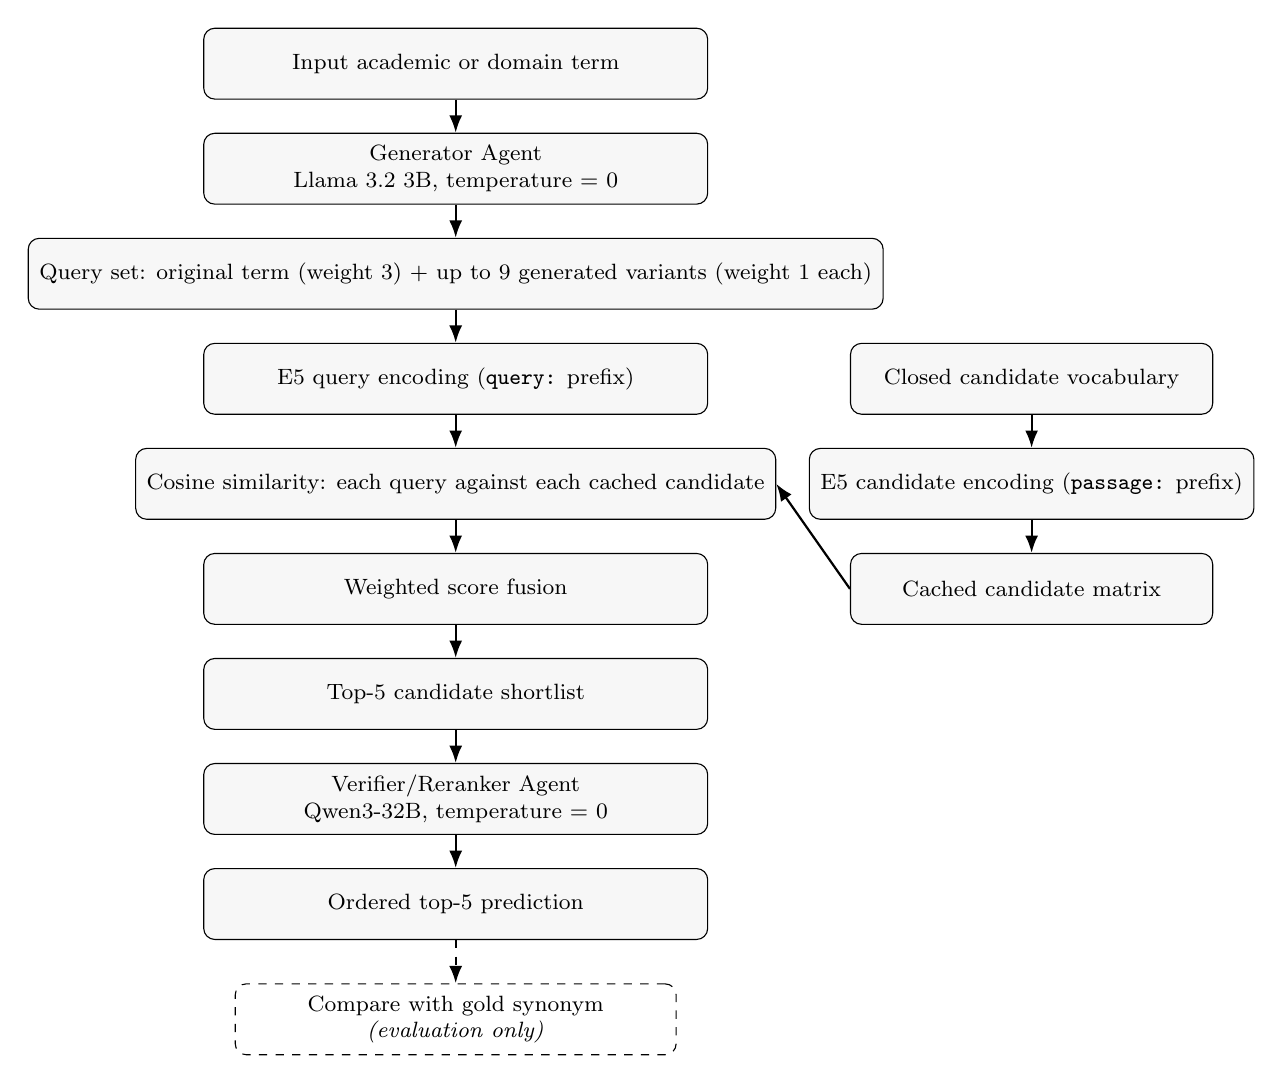
\begin{tikzpicture}[
  box/.style={draw, rounded corners, align=center, minimum width=6.4cm, minimum height=0.9cm, font=\footnotesize, fill=black!3, inner sep=4pt},
  sidebox/.style={draw, rounded corners, align=center, minimum width=4.6cm, minimum height=0.9cm, font=\footnotesize, fill=black!3, inner sep=4pt},
  evalbox/.style={draw, dashed, rounded corners, align=center, minimum width=5.6cm, minimum height=0.9cm, font=\footnotesize, inner sep=4pt},
  arr/.style={-{Latex[length=2.2mm]}, thick}
]
\node[box] (n1) {Input academic or domain term};
\node[box, below=0.42cm of n1] (n2) {Generator Agent\\ Llama 3.2 3B, temperature = 0};
\node[box, below=0.42cm of n2] (n3) {Query set: original term (weight 3) + up to 9 generated variants (weight 1 each)};
\node[box, below=0.42cm of n3] (n4) {E5 query encoding (\texttt{query:} prefix)};
\node[box, below=0.42cm of n4] (n5) {Cosine similarity: each query against each cached candidate};
\node[box, below=0.42cm of n5] (n6) {Weighted score fusion};
\node[box, below=0.42cm of n6] (n7) {Top-5 candidate shortlist};
\node[box, below=0.42cm of n7] (n8) {Verifier/Reranker Agent\\ Qwen3-32B, temperature = 0};
\node[box, below=0.42cm of n8] (n9) {Ordered top-5 prediction};
\node[evalbox, below=0.55cm of n9] (n10) {Compare with gold synonym\\ \textit{(evaluation only)}};

\node[sidebox, right=1.8cm of n4] (b1) {Closed candidate vocabulary};
\node[sidebox, below=0.42cm of b1] (b2) {E5 candidate encoding (\texttt{passage:} prefix)};
\node[sidebox, below=0.42cm of b2] (b3) {Cached candidate matrix};

\draw[arr] (n1) -- (n2);
\draw[arr] (n2) -- (n3);
\draw[arr] (n3) -- (n4);
\draw[arr] (n4) -- (n5);
\draw[arr] (n5) -- (n6);
\draw[arr] (n6) -- (n7);
\draw[arr] (n7) -- (n8);
\draw[arr] (n8) -- (n9);
\draw[arr, dashed] (n9) -- (n10);

\draw[arr] (b1) -- (b2);
\draw[arr] (b2) -- (b3);
\draw[arr] (b3.west) -- (n5.east);
\end{tikzpicture}%
}
\caption{Fixed-role, centrally orchestrated multi-agent pipeline. The candidate-vocabulary branch on the right is encoded once and cached; only the query branch on the left is recomputed per input term.}
\label{fig:fixed-pipeline}
\end{figure}

The Generator Agent is the first agent in the fixed-role MAS. It is an LLM-based query-expansion component. Query expansion is the process of transforming one search expression into several semantically related expressions so that different lexical realizations of the same concept can be retrieved. The generator receives one English academic or domain term and returns up to nine short paraphrases or related expressions. The original term is prepended by the orchestration code, producing at most ten retrieval queries.

The Generator Agent was implemented with Llama 3.2 3B through Ollama. The 3B Llama 3.2 model is intended for instruction-following, rewriting, tool use, and related local applications, making it suitable for constrained query expansion. A local model was selected to avoid a paid API call for every generated variant set and to preserve acceptable latency during repeated validation experiments. The selected local model runs at Q4\_K\_M quantization on the project's Ollama installation.

The generator temperature was initially set to 0.3. However, repeated runs showed approximately one to two percentage points of Hit@1 variation. It was therefore reduced to 0.0 so that comparisons between fusion weights and candidate counts would be less affected by sampling variation. Despite this setting, cross-process runs were not perfectly identical. Consequently, the Generator Agent is best characterized as nominally deterministic under temperature-zero decoding but empirically variable across independent runs.

The benefit of query expansion is improved lexical and semantic coverage. A synonym that is distant from the original term in embedding space may become close to one of the generated variants. However, every additional query also introduces an opportunity for semantic drift. For example, a generated phrase may represent a related concept, a broader category, or a different sense of the original term.

This is intentional at the generation stage because the generated expressions are retrieval probes rather than final predictions. The closed-pool retrieval and ranking stages determine the final candidate. For this reason, generated queries are not treated as equally reliable to the original input.

The retrieval and fusion stages form the deterministic center of the pipeline and are supporting components of the fixed-role MAS rather than agents. The retrieval component receives the original query and generated variants and converts each string into a 768-dimensional E5 vector. Candidate-pool entries are encoded separately and cached. A similarity matrix is then calculated in which each row corresponds to one query and each column corresponds to one candidate. This structure makes it possible to reuse the same matrix while comparing alternative fusion strategies.

Retrieval is implemented as an exhaustive NumPy dot product between the normalized query-embedding matrix and normalized candidate-embedding matrix. Because the candidate vocabulary contains 921 entries, exhaustive comparison provides exact cosine-similarity scores at low computational cost.

Four multi-query fusion strategies were evaluated: maximum score, arithmetic mean, Reciprocal Rank Fusion, and a weighted mean. Maximum fusion allowed one poor generated query to dominate the result. Reciprocal Rank Fusion similarly gave excessive influence to high-ranked but unreliable candidates because it operates on rank positions rather than score magnitudes. The weighted mean produced the strongest result.

Under this method, the original term receives weight 3, while each generated variant receives weight 1. The fused candidate score is:

\begin{equation}
S(c) = \frac{3\,s(q_0,c) + \sum_{i=1}^{m} s(q_i,c)}{3+m}
\label{eq:weighted-fusion}
\end{equation}

where $q_0$ is the original term, $q_i$ is a generated variant, $m$ is the number of variants, $c$ is a candidate synonym, and $s(q,c)$ is the cosine-similarity score.

The denominator does not affect candidate ordering when the number of queries is fixed, but it preserves the interpretation of the result as a weighted mean.

This method was selected because it preserves query diversity without allowing one generated variant to outvote the original term. The original input therefore remains the principal source of evidence, while the LLM-generated variants act as supporting retrieval signals. The component outputs the five candidates with the highest fused scores. Increasing this shortlist to 10 or 15 candidates improved candidate recall slightly but reduced Hit@1 after reranking because the larger lists introduced more plausible distractors.

Candidate vectors are cached because the candidate vocabulary remains fixed across queries. Only the incoming term and its generated variants therefore require new embedding computation. The cache stores candidate embeddings as float32 NumPy arrays. The cache identifier is derived from the embedder model name and the deduplicated candidate-pool size. This design reduces repeated embedding computation and keeps the marginal retrieval cost per term low after the candidate embeddings have been prepared.

\section{Verifier/Reranker Agent}

The Verifier/Reranker Agent is the second agent in the fixed-role, centrally orchestrated multi-agent pipeline. It acts as a listwise verification and ranking component. It receives the original term and exactly five candidates produced by the deterministic retrieval and fusion stages and returns the same candidates ordered from most to least likely synonym.

Unlike embedding retrieval, which evaluates candidates through vector similarity, listwise reranking allows the agent to compare the candidates jointly in the context of the original term. The Verifier/Reranker Agent is constrained to the supplied shortlist. If its output omits one of the supplied candidates, the missing candidate is appended according to its previous order so that retrieval recall is preserved.

The selected Verifier/Reranker Agent uses Qwen3-32B through OpenRouter. The official model card describes Qwen3-32B as a 32.8-billion-parameter causal LLM with instruction-following, reasoning, multilingual, and agent capabilities.

This model was selected after a controlled comparison with a local Qwen3.5-2B reranker. When the two models were applied to the same upstream top-five lists, the 2B model reduced validation Hit@1 from 0.784 to 0.768, whereas Qwen3-32B increased it to 0.851. The smaller model was also slower on the available machine, requiring approximately 13.2 seconds per term compared with approximately 9.1 seconds for the API-hosted model in the validation run.

This result shows that reranker capability, not merely model presence, drove the outcome: moving from the 2-billion-parameter to the 32-billion-parameter model raised validation Hit@1 by 8.3 percentage points (0.768 to 0.851), a substantially higher accuracy that the larger model's greater ranking capability explains directly. The latency comparison should be read separately from this accuracy result: the available local hardware, not parameter count, explains why the smaller local model was also slower than the API-hosted larger one. The local Qwen3.5-2B model runs at Q8\_0 quantization.

The Verifier/Reranker Agent is limited by the candidate shortlist supplied by the deterministic retrieval stage. Its main contribution is therefore improved ordering among already-retrieved candidates. Reranking can also damage an already-correct result. On the complete dataset, 136 retrieved cases improved after reranking, while 48 worsened; 43 of the 48 regressions were candidates that had already been correct at rank one before being demoted. Therefore, the reranker was net beneficial, but its decisions were not uniformly reliable.

Within the fixed-role MAS, the Verifier/Reranker Agent is conceptually distinct from the retrieval component. Retrieval determines which candidate strings enter the shortlist through deterministic similarity calculations, whereas the Verifier/Reranker Agent performs LLM-based semantic evaluation of that shortlist before the final prediction is produced.

\section{Dynamic tool-calling architecture}

The alternative architecture replaces fixed query generation and fusion with a tool-calling controller. Tool calling allows an LLM agent to invoke an external retrieval function, inspect the returned data, and decide whether another retrieval call is useful.

The implemented architecture contains a single dynamic retrieval-control agent. It receives an input term and access to a \texttt{retrieve\_candidates} tool. At runtime, the agent decides how many additional retrieval calls to perform and which query paraphrase to pass with each call. It then uses \texttt{finalize} to return an ordered top-five list.

This differs conceptually from the fixed-role, centrally orchestrated MAS. In the fixed-role architecture, the Generator Agent and Verifier/Reranker Agent have predefined specialized roles and deterministic orchestration code determines the execution sequence. In the dynamic architecture, a single controller agent determines the retrieval actions at runtime.

The term single-agent refers specifically to control of the dynamic retrieval process. In the controlled architecture comparison, the resulting candidate list was subsequently sent to the same Qwen3-32B reranker used by the fixed-role pipeline. This reranker remained a fixed downstream ranking stage and did not participate in control of the tool-calling search loop.

Figure~\ref{fig:dynamic-agent} illustrates this distinction. The central retrieval loop is controlled by one dynamic agent, while the final reranker remains a fixed post-processing component.

\begin{figure}[htbp]
\centering
\resizebox{\textwidth}{!}{%
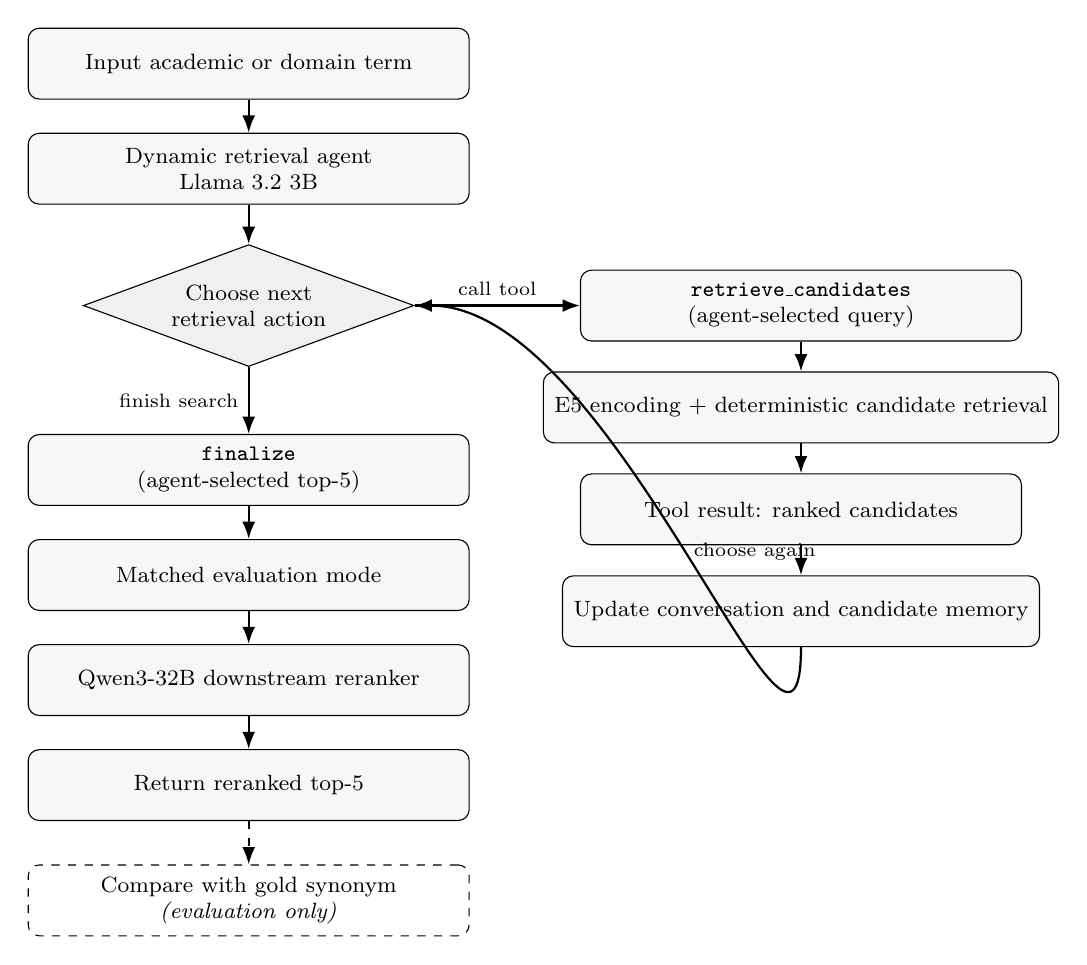
\begin{tikzpicture}[
  box/.style={draw, rounded corners, align=center, minimum width=5.6cm, minimum height=0.9cm, font=\footnotesize, fill=black!3, inner sep=4pt},
  decision/.style={draw, diamond, aspect=2.4, align=center, font=\footnotesize, fill=black!6, inner sep=2pt},
  evalbox/.style={draw, dashed, rounded corners, align=center, minimum width=5.6cm, minimum height=0.9cm, font=\footnotesize, inner sep=4pt},
  arr/.style={-{Latex[length=2.2mm]}, thick}
]
\node[box] (m1) {Input academic or domain term};
\node[box, below=0.42cm of m1] (m2) {Dynamic retrieval agent\\ Llama 3.2 3B};
\node[decision, below=0.5cm of m2, minimum width=4.2cm, minimum height=1.5cm] (m3) {Choose next\\ retrieval action};

\node[box, right=2.1cm of m3] (t1) {\texttt{retrieve\_candidates}\\ (agent-selected query)};
\node[box, below=0.38cm of t1] (t2) {E5 encoding + deterministic candidate retrieval};
\node[box, below=0.38cm of t2] (t3) {Tool result: ranked candidates};
\node[box, below=0.38cm of t3] (t4) {Update conversation and candidate memory};

\node[box, below=0.85cm of m3] (m4) {\texttt{finalize}\\ (agent-selected top-5)};
\node[box, below=0.42cm of m4] (m5) {Matched evaluation mode};
\node[box, below=0.42cm of m5] (m6) {Qwen3-32B downstream reranker};
\node[box, below=0.42cm of m6] (m7) {Return reranked top-5};
\node[evalbox, below=0.55cm of m7] (m8) {Compare with gold synonym\\ \textit{(evaluation only)}};

\draw[arr] (m1) -- (m2);
\draw[arr] (m2) -- (m3);
\draw[arr] (m3.east) -- node[above,font=\scriptsize]{call tool} (t1.west);
\draw[arr] (t1) -- (t2);
\draw[arr] (t2) -- (t3);
\draw[arr] (t3) -- (t4);
\draw[arr] (t4.south) to[out=270,in=0] node[right,font=\scriptsize]{choose again} (m3.east);
\draw[arr] (m3.south) -- node[left,font=\scriptsize]{finish search} (m4.north);
\draw[arr] (m4) -- (m5);
\draw[arr] (m5) -- (m6);
\draw[arr] (m6) -- (m7);
\draw[arr, dashed] (m7) -- (m8);
\end{tikzpicture}%
}
\caption{Dynamic tool-calling retrieval architecture. The agent may call \texttt{retrieve\_candidates} repeatedly before calling \texttt{finalize}; the downstream reranker is a fixed stage shared with the pipeline of Figure~\ref{fig:fixed-pipeline} in the matched comparison.}
\label{fig:dynamic-agent}
\end{figure}

The input to the dynamic controller was the same term used by the fixed system. Its intermediate outputs were tool calls containing model-selected query strings, while its final output was a top-five candidate list.

A deterministic safety mechanism anchors the search with the original input term before the agent begins its dynamic decisions. Finalization is constrained to candidate strings returned through retrieval. If the model reaches its turn budget before successfully finalizing, the accumulated retrieved candidate pool is used as the output. The turn budget is fixed at four turns.

The principal engineering benefit was adaptability. The agent could finish after the initial search, repeat retrieval with a paraphrase, or explore a different interpretation depending on the term. This behavior recovered five gold synonyms that were missed by the fixed pipeline during the matched validation comparison. For example, self-selected paraphrases sometimes identified candidate regions that were not reached by the fixed set of generated variants.

However, the same flexibility introduced less predictable control flow. The agent sometimes moved toward a plausible but incorrect sense, returned a weaker candidate set, or used additional planning calls without producing a corresponding accuracy improvement.

With the same E5 retriever and Qwen3-32B final reranker, the dynamic architecture achieved validation Hit@1 of 0.830 and average latency of 18.96 seconds per term. The fixed-role, centrally orchestrated multi-agent pipeline achieved validation Hit@1 of 0.851 at 9.08 seconds. The comparison therefore suggests that the dynamic search capability was real but did not provide a positive net trade-off for this dataset.

\section{Prompt and interface contracts}

The following contracts define the roles and interfaces of the LLM-based components used in the two architectures.

The Generator Agent belongs to the fixed-role, centrally orchestrated MAS and is configured as follows.

\paragraph{Generator Agent contract.}
Model: Llama 3.2 3B through Ollama.

\begin{lstlisting}[style=promptstyle]
System prompt:
"You are a domain terminology expert. Generate English synonyms or
closely related semantic variants for the given academic/domain term.
These variants will be used as search queries against a vocabulary
index, so include broader, narrower, and near-equivalent phrasings.
Return only a JSON list of short variants. Do not explain."

User message template:
Term: "{term}"
\end{lstlisting}

Production parameters:
\begin{itemize}
  \item temperature = 0.3 for the experimental configuration, or 0.0 for the final pipeline
  \item $n = 9$ for the final reranked pipeline; $n = 3$ for the faster local-only fallback
  \item the original input term is prepended by orchestration code
  \item local generation limit = 300 tokens
\end{itemize}

The Verifier/Reranker Agent is the second LLM agent in the fixed-role MAS.

\paragraph{Verifier/Reranker Agent contract.}
Model: Qwen3-32B through OpenRouter.

\begin{lstlisting}[style=promptstyle]
System prompt:
"You are a strict semantic ranking agent for domain terminology. You
receive one input term and a list of candidate synonyms. Your task is
to ORDER the candidates from best to worst according to semantic
equivalence. Do not invent new candidates. Do not remove candidates
unless they are completely invalid. Use the exact candidate strings
from the provided list. Return only a JSON list of candidate strings
ordered from best to worst."

User message template:
Term: "{term}"

Candidate synonyms:
1. {candidate_1}
2. {candidate_2}
...
\end{lstlisting}

Output constraints:
\begin{itemize}
  \item return only candidates present in the input list
  \item use the exact candidate strings supplied by the retrieval stage
  \item omitted candidates are appended in their previous order
\end{itemize}

Production parameters: temperature = 0.0.

The local reranker baseline uses the same ranking role and an almost identical prompt, with Qwen3.5-2B through Ollama and the local generation limit of 300 tokens.

The dynamic tool-calling architecture uses a separate single controller agent.

\paragraph{Dynamic tool-calling agent contract.}
Controller model: Llama 3.2 3B through native Ollama tool calling.

\begin{lstlisting}[style=promptstyle]
System prompt:
"You are a synonym-finding agent. You must find the best synonym for
a given term, choosing ONLY from a fixed vocabulary you can search
with the retrieve_candidates tool - you cannot invent candidates.
Call retrieve_candidates one or more times (try the term itself and,
if you think it will help, a paraphrase or a broader/narrower
phrasing) to gather good candidates. When you are confident, call
finalize with your final top 5 candidates ordered from best to worst,
using the exact candidate strings returned by retrieve_candidates.
Do not answer in plain text."
\end{lstlisting}

Production parameters:
\begin{itemize}
  \item temperature = 0.2
  \item max\_turns = 4
  \item the original input term is retrieved before the dynamic control loop begins
\end{itemize}

Tool schema --- \texttt{retrieve\_candidates}:

\begin{lstlisting}[style=jsonstyle]
{
  "type": "function",
  "function": {
    "name": "retrieve_candidates",
    "description": "Search the fixed candidate vocabulary for terms semantically close to a query. Returns up to top_k candidate strings, best match first.",
    "parameters": {
      "type": "object",
      "properties": {
        "query": {
          "type": "string",
          "description": "Search query - the term or a paraphrase of it."
        },
        "top_k": {
          "type": "integer",
          "description": "How many candidates to return (default 5, max 10)."
        }
      },
      "required": ["query"]
    }
  }
}
\end{lstlisting}

Tool schema --- \texttt{finalize}:

\begin{lstlisting}[style=jsonstyle]
{
  "type": "function",
  "function": {
    "name": "finalize",
    "description": "Submit the final ranked list of up to 5 candidate synonyms, best first. Must use exact strings previously returned by retrieve_candidates.",
    "parameters": {
      "type": "object",
      "properties": {
        "ranked_candidates": {
          "type": "array",
          "items": {
            "type": "string"
          },
          "description": "Up to 5 candidate strings, best synonym first."
        }
      },
      "required": ["ranked_candidates"]
    }
  }
}
\end{lstlisting}

Safety constraints are enforced by the orchestration code. Finalization accepts candidate strings originating from the retrieval tool, and the accumulated retrieved pool provides a deterministic fallback if the turn budget is reached.

\section{Engineering trade-offs and selection guidance}

The model progression shows that the largest engineering gains did not come from adding complexity indiscriminately. Instead, each useful stage addressed a specific limitation of the previous one. Replacing MiniLM with E5 improved the semantic representation at almost no latency cost. Adding the Generator Agent improved candidate recall and ranking by providing multiple lexical formulations for deterministic retrieval. Weighted fusion reduced the effect of semantic drift by preserving a larger contribution from the original query. Finally, the Verifier/Reranker Agent improved ordering among candidates that had already been retrieved.

Table~\ref{tab:tradeoffs} summarizes the principal operating points. The reported test value for the final pipeline is the fallback-verified rerun, because every candidate list in that execution was confirmed to have received a valid reranker response.

\begingroup
\footnotesize
\begin{table}[htbp]
\centering
\setlength{\tabcolsep}{3pt}
\begin{tabular}{p{3.0cm}p{1.1cm}p{1.1cm}p{2.2cm}p{2.6cm}p{2.6cm}}
\toprule
\textbf{Operating point} & \textbf{Test Hit@1} & \textbf{Test MRR} & \textbf{Approx.\ latency/term} & \textbf{Monetary API cost} & \textbf{Intended use}\\
\midrule
MiniLM embedding baseline & 0.536 & 0.629 & 0.022 s & None & Minimal-compute baseline\\
E5 embedding baseline & 0.603 & 0.704 & 0.025 s & None & Low-latency local retrieval\\
E5 with local query expansion and weighted fusion, no reranker & 0.768 & 0.835 & 0.72 s & None & Strong local-only configuration\\
Fixed-role, centrally orchestrated MAS with Qwen3-32B reranking & 0.830 & 0.884 & 13.32 s (fallback-verified test run) & Approx.\ \$0.03 per 194 terms & Highest confirmed accuracy\\
Dynamic tool-calling retrieval with Qwen3-32B reranking & 0.830 (val.) & 0.866 (val.) & 18.96 s & Approx.\ \$0.03 per 194 terms, same reranker call pattern & Experimental adaptive retrieval\\
\bottomrule
\end{tabular}
\caption{Principal operating points on the accuracy--latency--cost frontier. Values for the dynamic architecture are validation-split figures, as noted, since it was not run on the test split.}
\label{tab:tradeoffs}
\end{table}
\endgroup

These values show a clear accuracy-latency frontier rather than one universally preferable model. The E5 baseline is approximately 30 times faster than the local expansion pipeline, while the expansion pipeline is substantially faster and cost-free compared with API reranking. Conversely, the final Verifier/Reranker Agent produces an important improvement in top-one ordering, particularly when the correct synonym is already present in the shortlist.

The E5-only configuration should be preferred when latency, local execution, and operational simplicity are the principal requirements. It requires no generative stage and has negligible marginal cost once the candidate vectors are cached. However, its lower Hit@1 indicates that a single vector representation does not cover all lexical forms and domain-specific synonym relations present in the dataset.

The local expansion configuration should be preferred when API independence is required but a moderate latency increase is acceptable. It offers a substantial improvement over E5 alone and can be executed entirely with local models. Its principal risk is generator drift. Therefore, the original-term weight should remain greater than the weight assigned to each generated variant.

The complete fixed-role, centrally orchestrated multi-agent pipeline should be preferred for offline evaluation, catalogue construction, batch terminology processing, or other settings in which accuracy is more important than interactive response time. It provides the strongest confirmed result and follows a predictable execution sequence.

Its centralized orchestration also makes each stage independently observable: generated variants, embedding scores, fused rankings, and final reranker output can be logged separately. This structure improves traceability and makes failures easier to attribute to generation, retrieval, fusion, or reranking.

The dynamic tool-calling agent should be considered when terms vary substantially in difficulty and some inputs may benefit from adaptive search. Its ability to recover candidates missed by the fixed pipeline demonstrates that self-directed retrieval can produce complementary evidence. However, it should not be selected solely because it provides greater runtime control. Under the tested conditions, additional planning increased latency and produced more regressions than recoveries.

The distinction between the two architectures is therefore fundamental:

\begin{quote}
\textbf{Fixed-role, centrally orchestrated MAS:} a Generator Agent and Verifier/Reranker Agent have predefined specialized roles, while deterministic orchestration code controls a fixed execution sequence and deterministic retrieval/fusion components operate between the two agents.
\end{quote}

\begin{quote}
\textbf{Dynamic tool-calling architecture:} one controller agent determines retrieval queries and tool calls dynamically during execution, with the Qwen3-32B reranker retained as a fixed downstream stage in the matched comparison.
\end{quote}

The 2B local reranker should not be used in the final architecture. Its addition increased latency while reducing Hit@1 on a controlled upstream shortlist. This result demonstrates that reranking quality depends on model capability and task alignment. A reranker does not provide value merely because it processes the candidates jointly.

Finally, the candidate shortlist should remain small unless the reranker or retrieval strategy is changed. Increasing the pool from five to ten or fifteen candidates increased the probability that the gold synonym was available, but it also exposed the reranker to more semantically plausible distractors and reduced top-one accuracy. Therefore, shortlist width must be optimized jointly with reranker capability rather than treated only as a recall parameter.

\section{Methodology and evaluation protocol}
\label{sec:methodology}

This section defines the metrics used to score every configuration reported in this thesis. The Data chapter defines the dataset and the closed candidate vocabulary (Section~\ref{sec:candidate-vocab}); this section defines how a predicted ranking is turned into a number, so that the comparisons reported in the Results chapter rest on a single, explicit protocol.

For a given input term, a system returns an ordered list of candidates drawn from the closed vocabulary. Let $r_i$ denote the rank, within that ordered list, of the gold synonym recorded for row $i$, with $r_i = \infty$ if the gold synonym is absent from the returned list altogether. All metrics below are computed per row from $r_i$ and then averaged over the $N$ rows of the split being reported.

\subsection{Hit@\textit{k}}

Hit@$k$ is the proportion of rows for which the gold synonym is returned within the first $k$ positions:

\begin{equation}
\operatorname{Hit@}k = \frac{1}{N} \sum_{i=1}^{N} \mathbb{1}\!\left[r_i \leq k\right].
\label{eq:hit-at-k}
\end{equation}

This thesis reports Hit@1, Hit@3, and Hit@5. Hit@1 is treated as the primary metric, since it measures whether the system's single first-choice prediction is correct -- the intended mode of use for the system. Hit@3 and Hit@5 measure whether the gold synonym is present anywhere in a short shortlist, which is useful for separating a retrieval-coverage failure (the gold synonym is never shortlisted) from a ranking failure (it is shortlisted but not placed first); this distinction is used throughout the error analysis in the Results chapter.

\subsection{Mean Reciprocal Rank}

Mean Reciprocal Rank (MRR) averages the reciprocal of the gold synonym's rank, assigning zero credit when it is absent from the returned list:

\begin{equation}
\operatorname{MRR} = \frac{1}{N} \sum_{i=1}^{N}
\begin{cases}
1/r_i, & r_i < \infty,\\
0, & r_i = \infty.
\end{cases}
\label{eq:mrr}
\end{equation}

Unlike Hit@$k$, which is binary at a fixed cutoff, MRR gives partial, rank-sensitive credit. It distinguishes two systems that achieve the same Hit@5 but place the gold synonym at different average positions within the top five.

\subsection{Normalized Discounted Cumulative Gain}

Normalized Discounted Cumulative Gain at cutoff $k$ (NDCG@$k$) is a rank-sensitive metric that discounts a correct result logarithmically by its position. Under the single-relevant-item setting used in this thesis (each row has exactly one gold synonym, treated as a binary-relevant item), NDCG@$k$ for row $i$ reduces to:

\begin{equation}
\operatorname{NDCG@}k_i =
\begin{cases}
1/\log_2(r_i+1), & r_i \leq k,\\
0, & r_i > k,
\end{cases}
\label{eq:ndcg-at-k}
\end{equation}

averaged over rows to obtain the reported NDCG@3 and NDCG@5. NDCG@$k$ and MRR are related -- both discount by rank -- but are not identical, since their discount functions differ ($1/\log_2(r_i+1)$ versus $1/r_i$); NDCG@$k$ additionally saturates to zero outside its cutoff $k$, which MRR does not.

\subsection{Rank matching and reporting conventions}

The rank $r_i$ used in Equations~\ref{eq:hit-at-k}--\ref{eq:ndcg-at-k} is computed by normalized string equality between a candidate and the row's gold synonym (Section~\ref{sec:normalization} of the Data chapter), not literal character-for-character equality: a candidate differing from the gold value only in case or surface punctuation is scored as a match. Because each row provides exactly one gold label, these metrics do not give credit for an alternative, unrecorded synonym that may be equally valid (Section~\ref{sec:data-limitations}); this is a property of the annotation scheme rather than of the metrics themselves. Absolute hit counts are reported alongside proportions throughout the Results chapter, particularly for the 194-row validation and test splits, where a single changed prediction corresponds to approximately 0.52 percentage points.

\section{Chapter summary}

This chapter presented the model families and software components used for closed-pool synonym ranking. The selected system combines local LLM-based query expansion, E5 dense embeddings, deterministic weighted score fusion, and Qwen3-32B listwise verification and reranking.

The selected architecture is consistently characterized as a \textbf{fixed-role, centrally orchestrated multi-agent pipeline}. Its two LLM agents have distinct predefined responsibilities: the Generator Agent produces retrieval-oriented semantic variants, while the Verifier/Reranker Agent evaluates and reorders the candidate shortlist to produce the final prediction. E5 retrieval, cosine-similarity computation, candidate caching, and weighted fusion are deterministic supporting components rather than agents. Their execution and the transfer of information between stages are controlled by deterministic orchestration code.

In compact form:

\begin{quote}
\textbf{Fixed-role MAS = Generator Agent + Verifier/Reranker Agent, with retrieval and fusion used as deterministic tools.}
\end{quote}

The dynamic tool-calling alternative follows a different control structure. One dynamic controller agent selects retrieval actions at runtime and can adapt its search queries according to previous tool results. In the matched comparison, its candidate output was passed to the same Qwen3-32B downstream reranker used by the fixed architecture. Although the dynamic approach recovered some complementary candidates, the fixed-role, centrally orchestrated multi-agent pipeline achieved higher validation Hit@1 and substantially lower latency under the tested conditions.

Overall, the experimental progression indicates that performance improved when each additional component addressed a distinct error mode. E5 strengthened semantic retrieval, the Generator Agent increased retrieval coverage through multiple semantic formulations, deterministic weighted fusion limited the influence of noisy expansions, and the Verifier/Reranker Agent improved final ordering within a small candidate shortlist. This division of responsibilities provides the conceptual and engineering basis for the selected fixed-role, centrally orchestrated MAS.

\chapter{Results}
\label{chap:results}

\section{Executive summary}

This chapter reports the experimental results for the closed-pool synonym-ranking task. It summarizes the evaluation protocol and configurations, presents the progression from the original embedding baseline to the final retrieve-then-rerank pipeline, compares the fixed-role pipeline with the dynamic tool-calling agent under a matched downstream configuration, and analyzes the remaining errors, latency trade-offs, and statistical evidence.

The final fixed-role, centrally orchestrated multi-agent pipeline was executed on the held-out test split (194 rows) on two occasions. The execution treated as primary throughout this chapter is the one performed after explicit reranker-fallback tracking confirmed that every prediction used a genuine reranker response: Hit@1 = 0.830, Hit@3 = 0.938, Hit@5 = 0.948, MRR = 0.884, NDCG@3 = 0.896, NDCG@5 = 0.901. An earlier execution of the identical configuration, performed before fallback tracking existed and therefore not retrospectively verifiable, obtained Hit@1 = 0.851 and MRR = 0.892; it is retained in this chapter as direct evidence of run-to-run variability in the externally hosted reranker, not as a competing result.

On the same held-out split, the observed progression was: the original all-MiniLM-L6-v2 embedding baseline, Hit@1 = 0.536; replacing it with intfloat/e5-base-v2, Hit@1 = 0.603; adding local LLM-based query expansion and weighted multi-query fusion, Hit@1 = 0.768; adding Qwen3-32B reranking (the verified execution above), Hit@1 = 0.830.

On the complete 969-row dataset, used only for descriptive error analysis, the final configuration placed 797 gold synonyms at rank one (82.2\%), left 119 gold synonyms retrievable but not first-ranked (12.3\%), and failed to retrieve 53 gold synonyms at all (5.5\%). A matched downstream comparison, in which a dynamic tool-calling architecture was passed through the same Qwen3-32B reranker as the fixed-role pipeline, found that the fixed-role pipeline reached validation Hit@1 = 0.851 at 9.08 seconds per term, against Hit@1 = 0.830 at 18.96 seconds per term for the dynamic agent.

\section{Experimental context}

\subsection{Dataset, splits, and evaluation protocol}

The experiments use the 969-row evaluation dataset and the closed candidate vocabulary described in the Data chapter, partitioned by unique input term with seed 42 into 581 training, 194 validation, and 194 test rows (Section~\ref{sec:partitioning}). No component of the evaluated systems is trained with gradient descent; nevertheless, selecting an embedding model, fusion strategy, expansion width, reranker, or threshold from observed performance is itself a form of data-dependent decision-making. The validation split was used throughout the project for these decisions. The test split was not used for direct model or hyperparameter selection; several configurations already selected through validation were subsequently evaluated on it at different points during the project, including two executions of the final pipeline, discussed in Section~\ref{sec:threats}. The 969-row full dataset (train, validation, and test combined) is used only for descriptive reporting and error analysis after the final configuration had been selected; it is not an independent held-out sample.

\subsection{Metrics}

Predictions are scored with Hit@1, Hit@3, Hit@5, Mean Reciprocal Rank (MRR), and Normalized Discounted Cumulative Gain at cutoffs three and five (NDCG@3, NDCG@5). Hit@1 and MRR are prioritized in this chapter's interpretation, reflecting that the system's first proposed synonym is the primary intended output; Hit@5 and NDCG are used to separate retrieval-coverage failures from ranking-order failures in the error analysis (Section~\ref{sec:error-analysis}). Formal definitions of these metrics are given in the Methodology and Evaluation Protocol section of the Models chapter.

\subsection{Execution environment}

Local experiments were executed on an NVIDIA RTX 4050 Laptop GPU with approximately 6 GB of VRAM; concurrent local model executions were found to overload this GPU, so computationally intensive local runs were subsequently executed serially. Local query generation and the local reranker baseline ran through Ollama; Qwen3-32B reranking was executed remotely through OpenRouter.

\section{Main quantitative results}
\label{sec:main-results}

\subsection{Progression from baseline to final system}

Table~\ref{tab:test-progression} reports the main held-out test configurations. The configurations summarized here were selected through the development and validation process described in Section~\ref{sec:ablations}; their test results are reported retrospectively to characterize held-out performance, not as a sequence of decisions made by comparing test scores.

The original embedding baseline (all-MiniLM-L6-v2, single query) achieved test Hit@1 = 0.536, MRR = 0.629. Replacing it with intfloat/e5-base-v2 increased test Hit@1 to 0.603, MRR to 0.704, at an almost unchanged latency of approximately 0.025 seconds per term. Adding local LLM-based query expansion (temperature 0, weighted multi-query fusion) increased test Hit@1 to 0.768, MRR to 0.835, at approximately 0.72 seconds per term. Finally, reordering the resulting shortlist with Qwen3-32B produced the verified result already given in the executive summary (Hit@1 = 0.830, Hit@3 = 0.938, Hit@5 = 0.948, MRR = 0.884), at 13.32 seconds per term.

\begingroup
\footnotesize
\begin{table}[htbp]
\centering
\setlength{\tabcolsep}{4pt}
\begin{tabular}{p{4.4cm}p{0.7cm}p{1.0cm}p{1.0cm}p{1.0cm}p{1.0cm}p{1.6cm}}
\toprule
\textbf{Configuration} & \textbf{n} & \textbf{Hit@1} & \textbf{Hit@3} & \textbf{Hit@5} & \textbf{MRR} & \textbf{Latency/term}\\
\midrule
MiniLM embedding baseline & 194 & 0.536 & 0.722 & 0.773 & 0.629 & 0.022 s\\
E5 (e5-base-v2), single query & 194 & 0.603 & 0.789 & 0.871 & 0.704 & $\sim$0.025 s\\
E5 + local expansion + weighted fusion, $n=3$ & 194 & 0.768 & 0.902 & 0.933 & 0.835 & 0.72 s\\
E5 + expansion, temp.\ 0, $n=9$, no reranker & 194 & 0.747 & 0.907 & 0.948 & 0.827 & 0.72 s\\
Fixed-role pipeline + Qwen3-32B, original run & 194 & 0.851 & 0.923 & 0.949 & 0.892 & 9.27 s\\
Fixed-role pipeline + Qwen3-32B, fallback-verified run & 194 & 0.830 & 0.938 & 0.948 & 0.884 & 13.32 s\\
\bottomrule
\end{tabular}
\caption{Main held-out test results and experimental progression. The fallback-verified run is the primary reported test result throughout this chapter (Section~\ref{sec:threats}).}
\label{tab:test-progression}
\end{table}
\endgroup

Relative to the original baseline, the verified final pipeline improved test Hit@1 by approximately 29.4 percentage points (0.536 to 0.830); relative to the E5-only baseline, by approximately 22.7 percentage points. This gain in ranking quality is accompanied by a latency increase from approximately 0.025 seconds (E5 only) to 13.32 seconds (verified final pipeline) per term.

Two rows in Table~\ref{tab:test-progression} report an $n=3$ and an $n=9$ expansion-width configuration; the pre-reranking base of the final pipeline is the $n=9$, temperature-zero configuration, even though the $n=3$ configuration obtained a higher test Hit@1 (0.768 versus 0.747) without a reranker. The available results do not establish the specific reason $n=9$ was retained as the pre-reranking base for the final, reranked pipeline rather than $n=3$; this is an open question, noted here rather than resolved with an unsupported explanation.

\section{Validation ablations}
\label{sec:ablations}

More than 40 candidate configurations were compared on the validation split before the final configuration was selected, covering alternative embedders, lexical retrieval, Reciprocal Rank Fusion (RRF), multi-query fusion strategies, cross-encoder reranking, local and remote LLM reranking, candidate-shortlist width, confidence gating, and the dynamic tool-calling architecture (Section~\ref{sec:architectures}). Table~\ref{tab:ablations} reports a representative subset.

\begingroup
\footnotesize
\begin{table}[htbp]
\centering
\setlength{\tabcolsep}{4pt}
\begin{tabular}{p{4.2cm}p{0.9cm}p{0.9cm}p{0.9cm}p{1.2cm}p{4.0cm}}
\toprule
\textbf{Configuration} & \textbf{Hit@1} & \textbf{Hit@5} & \textbf{MRR} & \textbf{Latency} & \textbf{Note}\\
\midrule
BM25 only & 0.222 & 0.376 & 0.277 & 0.0002 s & Lexical matching alone is insufficient for this task\\
MiniLM baseline & 0.546 & 0.804 & 0.642 & 0.019 s & Original dense baseline\\
e5-base-v2 & 0.691 & 0.907 & 0.773 & 0.024 s & Strong, inexpensive baseline\\
E5 + BGE, RRF ensemble & 0.670 & 0.918 & 0.767 & 0.048 s & Higher Hit@5, lower Hit@1/MRR than E5 alone\\
Expansion + max fusion & 0.655 & 0.881 & 0.743 & 0.76 s & A single noisy variant can dominate\\
Expansion + mean fusion & 0.753 & 0.912 & 0.822 & 0.74 s & Below weighted fusion\\
Expansion + RRF & 0.629 & 0.887 & 0.728 & 0.72 s & Rank-based fusion underperformed\\
Expansion + weighted fusion, temp.\ 0.3 & 0.773 & -- & -- & -- & Initially adopted fusion strategy, before the temperature-zero retune\\
Expansion + weighted fusion, temp.\ 0 & 0.784 & 0.923 & 0.842 & 0.74 s & Strong pre-reranking configuration; base of the final pipeline\\
Weighted fusion + local 2B reranker & 0.768 & 0.923 & 0.837 & 13.21 s & Local reranker reduced Hit@1 relative to no reranking\\
Confidence-gated Qwen3-32B reranking & 0.835 & 0.923 & 0.873 & 3.78 s & Faster, but below blanket reranking\\
Weighted fusion + Qwen3-32B reranking & 0.851 & 0.923 & 0.882 & 9.08 s & Selected validation configuration\\
\bottomrule
\end{tabular}
\caption{Representative validation ablations. Hit@5, MRR, and latency are omitted for the temperature-0.3 weighted-fusion row where the available records report only Hit@1 for that configuration.}
\label{tab:ablations}
\end{table}
\endgroup

Two negative results were particularly informative for scoping the final design. Lexical retrieval alone (BM25) reached only Hit@1 = 0.222, and combining it with E5 consistently reduced Hit@1 relative to E5 alone; cross-encoder rerankers trained for general sentence similarity or duplicate-question detection similarly reduced performance, suggesting that general semantic relatedness was not a sufficient criterion for the stricter equivalence relation required by this task. A larger E5 variant (e5-large-v2) also performed substantially worse than e5-base-v2 under the tested implementation, indicating that embedding-model size alone did not predict task performance.

The multi-query fusion ablation shows that generated variants improved retrieval only when their contribution was controlled: maximum-score fusion (0.655) and RRF (0.629) underperformed the single-query E5 baseline (0.691), while mean fusion (0.753) and weighted fusion recovered and exceeded it. Table~\ref{tab:ablations} reports two weighted-fusion results that must not be read as a single configuration: 0.773 corresponds to the initially adopted weighted-fusion configuration, run with the query-expansion generator at temperature 0.3; 0.784 corresponds to the same fusion strategy after the generator was moved to temperature 0 for later controlled experiments (Section~\ref{sec:threats}), and is the configuration retained as the pre-reranking base of the final pipeline. In both configurations, the fusion weighted the original input term three times more strongly than each generated variant, which prevented an individually noisy paraphrase from dominating the ranking.

The reranker-size comparison is also informative. Reranking the same upstream shortlist, a local 2-billion-parameter reranker (Qwen3.5-2B) decreased validation Hit@1 from 0.784 to 0.768, while the 32-billion-parameter remote reranker (Qwen3-32B) increased it to 0.851. An intermediate 9-billion-parameter OpenRouter model was also attempted but did not yield a usable comparison, because repeated upstream provider-availability failures prevented a complete run; this attempt is not treated as a meaningful three-point model-size comparison in this chapter. Taken together, these results do not support the general claim that ``LLM reranking improves synonym ranking''; reranking was beneficial specifically when the reranking model was sufficiently capable under the tested prompt and candidate set, and harmful otherwise.

Reranker fallback tracking was introduced to ensure that failed API calls could not silently be treated as valid reranking outputs; every result reported in this chapter as ``verified'' or as a full-dataset run has zero recorded fallbacks.

\begin{figure}[htbp]
\centering
\resizebox{0.92\textwidth}{!}{%
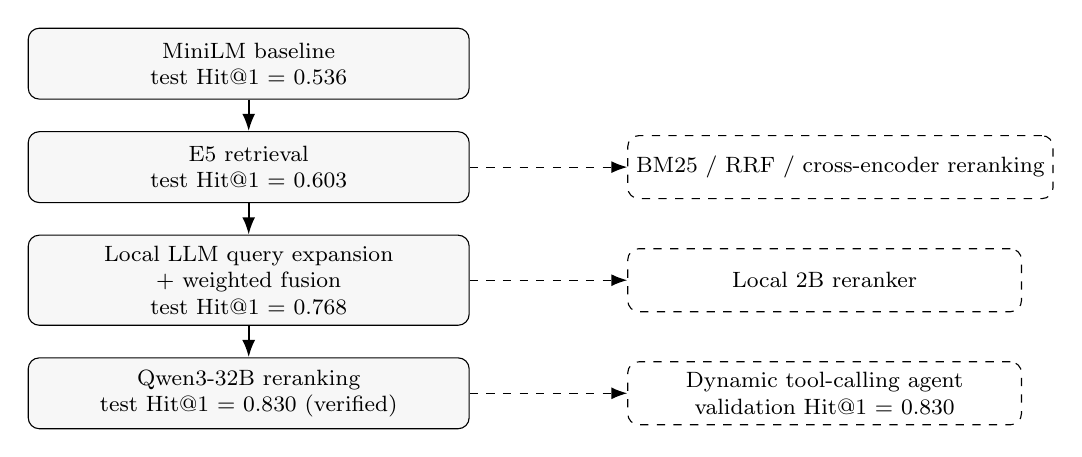
\begin{tikzpicture}[
  box/.style={draw, rounded corners, align=center, minimum width=5.6cm, minimum height=0.9cm, font=\footnotesize, fill=black!3, inner sep=4pt},
  altbox/.style={draw, dashed, rounded corners, align=center, minimum width=5.0cm, minimum height=0.8cm, font=\footnotesize, inner sep=3pt},
  arr/.style={-{Latex[length=2.2mm]}, thick},
  altarr/.style={-{Latex[length=2mm]}, dashed}
]
\node[box] (n1) {MiniLM baseline\\ test Hit@1 = 0.536};
\node[box, below=0.4cm of n1] (n2) {E5 retrieval\\ test Hit@1 = 0.603};
\node[box, below=0.4cm of n2] (n3) {Local LLM query expansion\\ + weighted fusion\\ test Hit@1 = 0.768};
\node[box, below=0.4cm of n3] (n4) {Qwen3-32B reranking\\ test Hit@1 = 0.830 (verified)};

\node[altbox, right=2.0cm of n2] (a1) {BM25 / RRF / cross-encoder reranking};
\node[altbox, right=2.0cm of n3] (a2) {Local 2B reranker};
\node[altbox, right=2.0cm of n4] (a3) {Dynamic tool-calling agent\\ validation Hit@1 = 0.830};

\draw[arr] (n1) -- (n2);
\draw[arr] (n2) -- (n3);
\draw[arr] (n3) -- (n4);
\draw[altarr] (n2) -- (a1);
\draw[altarr] (n3) -- (a2);
\draw[altarr] (n4) -- (a3);
\end{tikzpicture}%
}
\caption{Experimental evolution of the system. Solid arrows indicate the sequence of retained improvements (Table~\ref{tab:test-progression}); dashed branches indicate alternatives investigated at each stage (Table~\ref{tab:ablations}, Section~\ref{sec:architectures}) that were not selected.}
\label{fig:evolution}
\end{figure}

\section{Fixed-role multi-agent pipeline versus dynamic tool-calling architecture}
\label{sec:architectures}

The final system is a \textbf{fixed-role, centrally orchestrated multi-agent pipeline}. A Generator Agent, an LLM-based component, produces query variants and paraphrases; E5-based retrieval, similarity scoring, and weighted fusion -- deterministic supporting components, not agents -- combine these into a candidate shortlist; a Verifier/Reranker Agent, a second LLM-based component, evaluates and reorders that shortlist to produce the final prediction. The execution order and the role of each component are fixed by deterministic orchestration code. This architecture is referred to as the fixed-role pipeline, or equivalently the centrally orchestrated fixed-role multi-agent system (MAS), throughout the remainder of this chapter.

The dynamic tool-calling architecture is conceptually distinct: a single controller agent decides at runtime how many retrieval calls to issue and which query to submit at each step, rather than following a fixed expansion strategy. Retrieval remains a tool invoked by this controller, not an agent in its own right. In the comparison reported here, the controller's resulting candidate list was subsequently passed through the same Qwen3-32B reranker used by the fixed-role pipeline; this reranker was a fixed downstream stage and did not participate in, or control, the dynamic retrieval loop.

To enable a matched downstream comparison, both architectures used the same E5 retrieval model and the same Qwen3-32B final reranker. This comparison controls the downstream retrieval and reranking models, but it is not compute-matched: the dynamic controller can execute additional decision and tool-calling steps that the fixed pipeline does not perform, which is reflected in its higher latency (Section~\ref{sec:latency}).

On the validation split, the fixed-role pipeline achieved Hit@1 = 0.851, Hit@3 = 0.912, Hit@5 = 0.923, MRR = 0.882 (165/194 exact rank-one predictions); the dynamic architecture achieved Hit@1 = 0.830, Hit@3 = 0.907, Hit@5 = 0.907, MRR = 0.866 (161/194). The candidate sets produced by the two architectures were inspected for the rows where the dynamic architecture regressed relative to the fixed pipeline: none of the ten inspected regressions shared the same candidate set as the fixed pipeline, which is evidence that altered retrieval behavior, rather than reranker sampling variation alone, contributed to the observed differences; this inspection covered ten rows and is not a claim about the cause of every regression.

Four distinct types of row-level change were observed between the two architectures, and are kept terminologically separate here:

\begin{itemize}
  \item \textbf{Candidate-set recovery}: the gold candidate, absent from the fixed pipeline's shortlist, became present in the dynamic architecture's shortlist. Five such recoveries were observed.
  \item \textbf{Ranking correction}: the gold candidate was present in both shortlists but reached rank one only under the dynamic architecture. Seven such corrections were observed.
  \item \textbf{Ranking regression}: a row correct at rank one under the fixed pipeline was no longer correct at rank one under the dynamic architecture. Fourteen such regressions were observed.
  \item \textbf{Retrieval miss introduced}: a row that was a ranking error under the fixed pipeline (gold present but not rank one) became a retrieval miss under the dynamic architecture (gold absent from the shortlist). One such case was observed.
\end{itemize}

These four counts are not mutually exclusive contributions to a single arithmetic reconciliation of the aggregate Hit@1 change; they describe different row-level outcomes observed in the same comparison. The net effect is that validation Hit@1 moved from 165/194 (0.851) under the fixed pipeline to 161/194 (0.830) under the dynamic architecture, a net change of four rank-one predictions.

This outcome does not indicate that dynamic tool use is intrinsically inferior to a fixed pipeline. Under the tested dataset, prompts, local generator model, retrieval tool, and latency budget, the fixed expansion strategy produced a better balance between recovering missed candidates and preserving already-correct predictions. The dynamic agent's self-directed paraphrases occasionally reached candidates unavailable to the fixed strategy, but could also drift toward a related, non-equivalent sense of the input term -- a risk that is particularly consequential in closed-pool synonym ranking, where semantically associated but incorrect candidates are frequently available in the pool.

\section{Accuracy--latency trade-off}
\label{sec:latency}

Table~\ref{tab:latency} reports latency and approximate sequential throughput for the main configurations. Throughput values are the reciprocal of the recorded sequential per-term latency and should not be interpreted as measured parallel-serving capacity.

\begingroup
\footnotesize
\begin{table}[htbp]
\centering
\setlength{\tabcolsep}{4pt}
\begin{tabular}{p{4.0cm}p{1.3cm}p{0.9cm}p{0.9cm}p{1.4cm}p{2.6cm}}
\toprule
\textbf{Configuration} & \textbf{Split} & \textbf{Hit@1} & \textbf{MRR} & \textbf{Latency/term} & \textbf{Approx.\ sequential throughput}\\
\midrule
MiniLM baseline & test & 0.536 & 0.629 & 0.022 s & 45.5 terms/s\\
E5 only & test & 0.603 & 0.704 & 0.025 s & 40.0 terms/s\\
Expansion $n=3$, no reranker & test & 0.768 & 0.835 & 0.72 s & 1.39 terms/s\\
Fixed pipeline + Qwen3-32B, original run & test & 0.851 & 0.892 & 9.27 s & 0.108 terms/s\\
Fixed pipeline + Qwen3-32B, verified run & test & 0.830 & 0.884 & 13.32 s & 0.075 terms/s\\
Fixed pipeline + Qwen3-32B & validation & 0.851 & 0.882 & 9.08 s & 0.110 terms/s\\
Dynamic agent + Qwen3-32B & validation & 0.830 & 0.866 & 18.96 s & 0.053 terms/s\\
\bottomrule
\end{tabular}
\caption{Accuracy--latency trade-off for representative configurations.}
\label{tab:latency}
\end{table}
\endgroup

The dynamic architecture required approximately 2.1 times the wall-clock time per term of the fixed pipeline (18.96 s versus 9.08 s) for slightly lower validation accuracy. The additional latency is consistent with the extra controller decision steps and repeated retrieval interactions performed by the dynamic architecture before the shared final reranking stage; stage-level timings were not separately measured, so this should be read as a plausible attribution rather than a decomposed latency measurement.

The local-versus-remote reranker comparison illustrates that parameter count alone does not predict latency: the local 2-billion-parameter reranker required approximately 13.2 seconds per validation term, more than the remote 32-billion-parameter reranker's approximately 9.1 seconds. The two rerankers ran on different infrastructure (a local 6 GB GPU versus a remote, provider-routed API), so this comparison reflects serving infrastructure and routing at least as much as it reflects model size.

\section{Error analysis}
\label{sec:error-analysis}

\subsection{Failure decomposition}

The selected configuration was evaluated over the complete 969-row dataset for descriptive error analysis. Table~\ref{tab:failure-decomposition} reports the outcome of every row under two neutral definitions: a \emph{ranking error} is a row in which the gold candidate is present in the final top-five ranking but not at rank one; a \emph{retrieval miss} is a row in which the gold candidate is absent from the top-five shortlist altogether. This decomposition separates failures of shortlist coverage from failures of final candidate ordering, without attributing a ranking error to a specific component by default.

\begingroup
\footnotesize
\begin{table}[htbp]
\centering
\begin{tabular}{lrrp{5.4cm}}
\toprule
\textbf{Outcome} & \textbf{Count} & \textbf{Rate} & \textbf{Definition}\\
\midrule
Correct at rank 1 & 797 & 82.2\% & Gold candidate ranked first.\\
Ranking error & 119 & 12.3\% & Gold candidate present in the top five, not ranked first.\\
Retrieval miss & 53 & 5.5\% & Gold candidate absent from the top five.\\
\midrule
Total & 969 & 100\% & \\
\bottomrule
\end{tabular}
\caption{Failure decomposition on the complete 969-row dataset, selected final configuration.}
\label{tab:failure-decomposition}
\end{table}
\endgroup

Among the 119 ranking errors, the gold candidate was at rank 2 in 87 cases, rank 3 in 19 cases, rank 4 in 11 cases, and rank 5 in 2 cases: most ranking errors are close decisions rather than severe misorderings. Several are consistent with a semantically defensible but non-matching top choice -- for example, \emph{investment} (gold \emph{investing}) ranked first as \emph{funding}, and \emph{mediation} (gold \emph{conflict resolution}) ranked first as \emph{dispute resolution}.

Retrieval misses present a different pattern: examples include \emph{philosophy} $\rightarrow$ \emph{wisdom}, \emph{gospels} $\rightarrow$ \emph{good news}, \emph{information technology} $\rightarrow$ \emph{IT}, and \emph{identity management} $\rightarrow$ \emph{IdM}, spanning register shifts, semantically distant phrasings, and abbreviation-direction effects. Because the gold candidate never reaches the reranking stage in these rows, increasing reranker capability alone cannot resolve them.

\subsection{Failure rate by term type and lexical overlap}

Table~\ref{tab:term-type-failure} reports ranking-error and retrieval-miss rates by the heuristic term-type categories defined in the Data chapter (Section~\ref{sec:normalization}). Single-word terms show the highest rate on both failure types; their retrieval-miss rate (9.9\%) is more than twice that of compound terms (3.2\%) and multi-word phrases (4.4\%). These categories are project-specific heuristics rather than a curated linguistic taxonomy and should be read as exploratory diagnostics.

\begingroup
\footnotesize
\begin{table}[htbp]
\centering
\begin{tabular}{lrr}
\toprule
\textbf{Term type} & \textbf{Ranking-error rate} & \textbf{Retrieval-miss rate}\\
\midrule
Abbreviation-like & 5.9\% & 8.8\%\\
Compound & 11.3\% & 3.2\%\\
Multi-word phrase & 12.8\% & 4.4\%\\
Single word & 14.2\% & 9.9\%\\
\bottomrule
\end{tabular}
\caption{Failure rates by term type, complete 969-row dataset, selected final configuration.}
\label{tab:term-type-failure}
\end{table}
\endgroup

A post-hoc lexical-overlap indicator (Jaccard similarity between the whitespace-separated tokens of the input term and its gold synonym) shows a similar pattern: rows with no shared tokens (Jaccard similarity of 0) had a retrieval-miss rate of 8.9\% and a ranking-error rate of 16.0\%, compared with 1.7\% and 6.9\% respectively for rows with a Jaccard similarity above 0.33. This suggests that surface-level lexical distance between input and gold is associated with both failure types, though the mechanism is not established beyond this observed association.

\subsection{Effect of reranking}

A before-and-after comparison was performed on the 916 full-dataset rows for which the gold candidate had already been retrieved prior to the final Qwen3-32B reranking stage. Of these rows, 136 improved in gold rank, 732 were unchanged, and 48 worsened after reranking: reranking produced a positive net movement in gold rank across these rows. This is a statement about rank movement, not directly about Hit@1 counts, since not every improvement in rank corresponds to a new rank-one success. The regressions are not evenly distributed: 43 of the 48 worsened cases had been correct at rank one before reranking and were demoted afterward.

\begin{figure}[htbp]
\centering
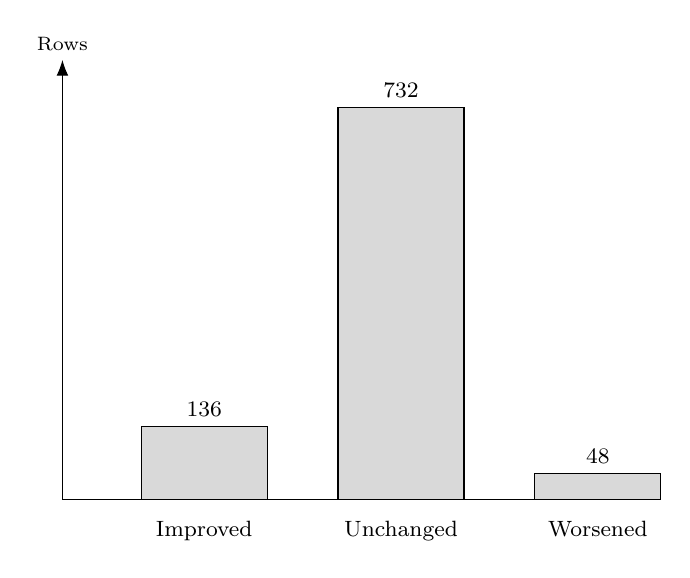
\begin{tikzpicture}[font=\footnotesize]
\def\scale{0.0068}
\draw[-{Latex[length=2mm]}] (0,0) -- (0,732*\scale+0.6) node[above,font=\scriptsize]{Rows};
\draw (0,0) -- (7.5,0);
\foreach \x/\lbl/\val in {1/Improved/136, 3.5/Unchanged/732, 6/Worsened/48} {
  \pgfmathsetmacro{\h}{\val*\scale}
  \draw[fill=black!15,draw=black] (\x,0) rectangle ++(1.6,\h);
  \node[above] at (\x+0.8,\h) {\val};
  \node[below] at (\x+0.8,-0.15) {\lbl};
}
\end{tikzpicture}
\caption{Gold-rank movement after Qwen3-32B reranking, on the 916 full-dataset rows where the gold candidate had already been retrieved. 43 of the 48 worsened rows had been correct at rank one before reranking.}
\label{fig:rerank-movement}
\end{figure}

This finding is consistent with why confidence-gated reranking did not outperform blanket reranking in validation. The gated configuration invoked Qwen3-32B only when the retrieval margin appeared ambiguous, reducing average validation latency from 9.08 to 3.78 seconds but also reducing Hit@1 from 0.851 to 0.835 (Table~\ref{tab:ablations}). Under the tested gating threshold, retrieval confidence was not sufficiently aligned with the cases in which reranking improved final ordering; this conclusion is limited to the tested threshold and reranker, not a general claim about confidence-gating strategies.

\subsection{Representative examples}

Replacing MiniLM with E5 recovered several rank-one predictions, including \emph{citizenship} $\rightarrow$ \emph{nationality}, \emph{feminism} $\rightarrow$ \emph{women's liberation}, \emph{brain} $\rightarrow$ \emph{cerebrum}, and \emph{fiscal policy} $\rightarrow$ \emph{budgetary policy}. These examples are consistent with E5 better capturing the intended semantic relation than MiniLM in these cases, rather than a lexically or topically related but non-equivalent candidate.

Query expansion produced further recoveries, for example \emph{stocks} $\rightarrow$ \emph{shares}, \emph{consciousness} $\rightarrow$ \emph{awareness}, and \emph{democracy} $\rightarrow$ \emph{popular government}, where a generated variant moved the gold candidate toward rank one. Expansion could also introduce plausible distractors: for \emph{investment}, fusion could favor \emph{funding} over the gold \emph{investing}; for \emph{sustainable tourism}, \emph{eco-tourism} could outrank the gold \emph{eco-friendly tourism}.

Qwen3-32B reranking corrected several such cases on validation, for example \emph{investment} (\emph{funding} $\to$ the gold \emph{investing}) and \emph{jurisprudence} (\emph{legal philosophy} $\to$ the gold \emph{legal theory}). The full-dataset analysis also recorded the reverse: for \emph{computer simulation}, the correct \emph{computational modeling} was demoted after reranking. Taken together, these examples are consistent with the reranking stage acting as a probabilistic ranking component rather than a deterministic arbiter of semantic correctness.

\section{Statistical interpretation}

\subsection{Confidence intervals}

Because Hit@$k$ is a binary outcome per row, 95\% Wilson score intervals were computed directly from the observed hit counts for the principal Hit@1 results (Table~\ref{tab:wilson}). The Wilson interval is appropriate for binomial proportions and behaves better than a normal approximation at finite sample sizes.

\begingroup
\footnotesize
\begin{table}[htbp]
\centering
\begin{tabular}{p{5.0cm}p{1.6cm}p{1.1cm}p{2.0cm}}
\toprule
\textbf{Configuration} & \textbf{Correct/n} & \textbf{Hit@1} & \textbf{95\% Wilson CI}\\
\midrule
MiniLM baseline, test & 104/194 & 0.536 & [0.466, 0.605]\\
E5 baseline, test & 117/194 & 0.603 & [0.533, 0.669]\\
Expansion $n=3$, test & 149/194 & 0.768 & [0.704, 0.822]\\
Final pipeline, original test run & 165/194 & 0.851 & [0.794, 0.894]\\
Final pipeline, verified test run & 161/194 & 0.830 & [0.771, 0.876]\\
Final pipeline, validation & 165/194 & 0.851 & [0.794, 0.894]\\
Final pipeline, full dataset (descriptive) & 797/969 & 0.822 & [0.797, 0.845]\\
\bottomrule
\end{tabular}
\caption{95\% Wilson confidence intervals for Hit@1. The full-dataset row is a descriptive interval over train, validation, and test combined, not an independent held-out interval.}
\label{tab:wilson}
\end{table}
\endgroup

For the verified test run, Hit@3 (182/194) has an approximate 95\% Wilson interval of [0.895, 0.964], and Hit@5 (184/194) of [0.908, 0.972]; both intervals are clearly above the corresponding Hit@1 interval, reinforcing that candidate-set recall at five items is substantially more reliable than exact rank-one accuracy. Confidence intervals for MRR and NDCG are not reported in this chapter, since a defensible interval for these metrics requires bootstrapping over per-row values rather than the aggregate means alone.

\subsection{Significance testing}

For the validation comparison between the temperature-zero expansion pipeline without reranking and the same pipeline with Qwen3-32B reranking, 16 terms moved from incorrect to correct and 3 moved from correct to incorrect; an exact two-sided McNemar test on these 19 discordant rows gives $p \approx 0.0044$. Because this comparison is performed on the same validation split used throughout the project for configuration selection, this $p$-value is best interpreted as descriptive paired evidence that the two configurations differ, rather than as an independent confirmatory significance test.

A second paired comparison is available between the original execution of the full reranked pipeline and the $n=3$ reranker-free configuration on test: 21 cases improved and 5 regressed, giving an exact two-sided McNemar value of $p \approx 0.0025$. Because these two configurations differ in both the reranking stage and the upstream expansion width (n=9 for the reranked pipeline versus n=3 for the baseline), this result is reported as a paired comparison between the two complete configurations, not as an isolated estimate of the effect of reranking. A corresponding paired significance test for the fallback-verified execution against these baselines is not available from the aggregate results reported here.

The validation difference between the fixed-role pipeline and the dynamic architecture (0.851 versus 0.830, Section~\ref{sec:architectures}) corresponds to approximately four additional rank-one successes over 194 rows. The candidate-set inspection in Section~\ref{sec:architectures} provides mechanistic evidence that the two architectures behave differently, but the available aggregates do not support a formal significance claim for this specific Hit@1 difference. The appropriate reading is that the fixed pipeline performed better under the tested conditions, not that it has been shown to be universally superior to dynamic-agent retrieval.

\section{Threats to validity}
\label{sec:threats}

\textbf{Sample size.} The held-out test split contains 194 rows, sufficient to distinguish large improvements, such as the change from MiniLM (Hit@1 = 0.536) to the verified final pipeline (Hit@1 = 0.830), but with limited resolution for configurations separated by one or two percentage points, as shown by the overlapping intervals in Table~\ref{tab:wilson}.

\textbf{Repeated use of one validation split.} Approximately 40 configurations were compared on the same 194-row validation split. Repeated experimentation on one split, even without direct test-set optimization, can adapt engineering decisions to peculiarities of that particular sample; this limits confidence in the exact ranking of configurations that differ by only a small margin.

\textbf{Reranker nondeterminism.} The final configuration was nominally identical, including temperature zero, across two separate test executions performed at different times, yet Hit@1 changed from 0.851 to 0.830 and average latency from 9.27 to 13.32 seconds per term. This variability is attributed to the externally hosted, provider-routed reranker rather than to any change in the pipeline code between the two runs, and it is the reason the more recent, fallback-verified execution -- confirmed free of silent reranker fallbacks -- is treated as the primary reported test result, while the earlier execution is retained as evidence of this variability. Future work should repeat this configuration several times to quantify this variability directly, rather than relying on two isolated executions.

\textbf{External-service dependence.} The best-performing configuration requires a paid, remotely hosted reranker (Qwen3-32B via OpenRouter), introducing network availability, provider availability, and pricing as operational dependencies that the E5-only and local-expansion alternatives do not share.

\textbf{Single-gold-label evaluation.} Exact matching against one designated gold synonym per row can penalize plausible alternatives, as seen in ranking errors such as \emph{eco-tourism} versus the gold \emph{eco-friendly tourism}, or \emph{dispute resolution} versus the gold \emph{conflict resolution}. The reported metrics therefore measure agreement with this dataset's specific synonym annotation, within the closed-pool ranking task as defined, rather than an unconstrained human judgment of synonym acceptability.

\textbf{Prompt sensitivity.} The generator and reranker prompt wording was not systematically varied under a controlled design, even though model choice, embedding model, fusion strategy, expansion count, temperature, shortlist width, and reranker strategy were. This remains an unexamined source of configuration sensitivity.

\section{Chapter summary}

Under the tested conditions, stronger dense retrieval, controlled LLM-based query expansion, and Qwen3-32B reranking each contributed to higher observed ranking performance, at the cost of progressively higher latency: test Hit@1 rose from 0.536 (MiniLM) to 0.603 (E5) to 0.768 (local expansion and weighted fusion) to 0.830 (verified fixed-role pipeline with Qwen3-32B reranking), while latency rose from approximately 0.022 seconds to 13.32 seconds per term. On the complete dataset, the final configuration ranked 82.2\% of gold synonyms first, left 12.3\% retrievable but not first-ranked, and failed to retrieve 5.5\%; reranking produced a positive net movement in gold rank but also demoted 43 previously correct rank-one predictions. A matched downstream comparison found that a dynamic tool-calling architecture, using the same retrieval model and reranker, did not exceed the fixed-role pipeline's accuracy and required roughly twice the latency. These conclusions are limited to the evaluated dataset, splits, and configurations described in this chapter.

\chapter{Conclusions}
\label{chap:conclusions}

\section{Executive summary}

This chapter synthesizes the project's findings from an applied software-engineering perspective. It restates the research questions in terms of the experiments actually performed, reviews the methodological choices that defined the final system, interprets the quantitative results together with their latency and reproducibility implications, and discusses the principal limitations and future work.

The project addressed synonym identification for English academic and domain-specific terms as a closed-pool ranking problem: given an input term, the system ranks candidates from a predefined vocabulary and places the corresponding gold synonym as high as possible. This formulation differs from unrestricted synonym generation because the final answer must belong to the fixed candidate vocabulary; even methods that free-generate a proposal with a language model ultimately use that text as a retrieval query and return a candidate from the controlled vocabulary.

Under these conditions, the strongest configuration was not the one with the greatest agent autonomy. The best-performing system combined a fixed-role, centrally orchestrated multi-agent pipeline with deterministic semantic retrieval and a constrained LLM reranking stage: a local generator based on Llama 3.2 3B, semantic representations from intfloat/e5-base-v2, weighted multi-query fusion, and Qwen3-32B as an external reranker. On the fallback-verified held-out test evaluation, this configuration achieved Hit@1 = 0.830, Hit@3 = 0.938, Hit@5 = 0.948, and MRR = 0.884.

The main engineering conclusion is therefore more specific than ``LLMs improve synonym ranking.'' LLMs were useful when assigned narrow, well-controlled responsibilities, while deterministic retrieval remained responsible for candidate grounding: LLM-based query expansion improved the retrieval stage, and a sufficiently capable reranker improved the ordering of already-retrieved candidates. Weaker rerankers, wider candidate pools, lexical fusion, and increased agent autonomy did not consistently improve the system. This is compatible with prior work showing that LLM-generated query expansions can strengthen dense retrieval, and supports the broader principle that tool use and generation should be evaluated as components rather than assumed to be beneficial by themselves.

These conclusions are bounded by the evaluated setting: one dataset, one predefined candidate vocabulary, one grouped split with a single fixed random seed, and a partially nondeterministic external reranking service. Paired significance testing (Section~\ref{sec:results-interpretation}) supports the largest observed differences; smaller differences, including the fixed-versus-dynamic architecture comparison, should be read with the corresponding caveats rather than as proven general superiority.

\section{Objectives and research questions}

The overall objective was to design and evaluate a practical system for identifying the intended synonym of an academic or domain-specific English term from a predefined vocabulary, investigating whether increasingly sophisticated retrieval and LLM-based components could improve ranking quality while maintaining explicit control over leakage, latency, and reproducibility. Approximately forty candidate configurations were explored through a common evaluation harness (Section~\ref{sec:ablations} of the Results chapter) rather than through isolated demonstrations.

Table~\ref{tab:research-questions} restates, as an operational summary, what the experiments tested and the conclusion each one supports.

\begingroup
\footnotesize
\begin{table}[htbp]
\centering
\begin{tabular}{p{5.6cm}p{7.4cm}}
\toprule
\textbf{Research question} & \textbf{Conclusion supported by the experiments}\\
\midrule
Can semantic retrieval and LLM-assisted query expansion improve closed-pool synonym ranking compared with a simple embedding baseline? & Yes, under the tested conditions. Replacing MiniLM with E5 improved the baseline substantially, and adding weighted LLM query expansion produced a further large improvement.\\
Does LLM reranking improve the ordering of retrieved synonym candidates, and does reranker capability matter? & Yes, but not universally. The local 2-billion-parameter reranker reduced performance, whereas the 32-billion-parameter Qwen3-32B reranker produced the strongest observed results.\\
Does a dynamic tool-calling agent outperform a fixed-role pipeline when downstream retrieval and reranking components are matched? & No, in the reported validation comparison. The dynamic agent recovered some complementary candidates but had lower aggregate accuracy and approximately twice the latency of the fixed-role pipeline.\\
\bottomrule
\end{tabular}
\caption{Research questions and the conclusions supported by the experiments.}
\label{tab:research-questions}
\end{table}
\endgroup

\subsection{Retrieval and query expansion}

This question is supported by a clear experimental progression. The original all-MiniLM-L6-v2 baseline reached test Hit@1 = 0.536. Replacing it with e5-base-v2 increased Hit@1 to 0.603. LLM query expansion combined with weighted E5 retrieval then increased Hit@1 to 0.768 in the best local-only configuration; a strong reranker further increased the fallback-verified result to 0.830. The use of E5 is consistent with its design as a general-purpose dense retrieval model, and the use of LLM-generated query variants is consistent with prior work showing that generated expansions can improve dense retrieval.

\subsection{Reranker capability}

This question produced a positive result together with an important negative one: a reranker is not beneficial simply because it is LLM-based. In the controlled validation comparison, a local, 2-billion-parameter reranker (Qwen3.5-2B) reduced Hit@1 from 0.784 to 0.768 on the same upstream retrieval configuration, whereas Qwen3-32B increased it to 0.851. The useful contribution was not reranking in the abstract, but reranking with a model sufficiently capable of distinguishing strict synonymy from broader semantic relatedness.

\subsection{Fixed-role pipeline versus dynamic tool-calling agent}

The dynamic tool-calling architecture allowed a controller agent to decide how often retrieval should be invoked and which paraphrases to search, in the spirit of tool-selection behavior studied in ReAct and Toolformer. When both architectures were evaluated with E5 retrieval and the same Qwen3-32B reranker, the fixed-role pipeline reached Hit@1 = 0.851 and MRR = 0.882 on validation, compared with 0.830 and 0.866 for the dynamic agent, at average latencies of 9.08 and 18.96 seconds per term respectively.

This comparison should be read precisely. The fixed architecture is a fixed-role, centrally orchestrated multi-agent pipeline: a Generator Agent and a Verifier/Reranker Agent perform specialized LLM-based tasks, but orchestration is centralized and deterministic -- the agents do not negotiate, allocate tasks among themselves, or dynamically define the execution graph. The project therefore demonstrates the value of specialized agents embedded in a controlled pipeline for this task, not a general advantage of decentralized multi-agent reasoning over agentic control in general.

\section{Methodological synthesis}

Four methodological decisions are particularly important for interpreting the results: the task was formulated as closed-pool, transductive synonym ranking; data partitions were grouped by input term; the candidate vocabulary was separated conceptually from row-specific ground truth; and system selection was performed on validation rather than directly on test results.

The evaluation dataset contained 969 rows after one degenerate identity pair was removed, partitioned into 581 training, 194 validation, and 194 test rows with a fixed seed of 42, grouped by unique input term rather than independently by row. This grouping prevents a duplicated input term with more than one valid synonym from appearing across different partitions with different gold labels.

The global candidate vocabulary was constructed from synonym values across the prepared dataset. Under the closed-pool task as defined, this is not label leakage: the system is allowed to know the vocabulary of possible answers, and what is prohibited is consulting the gold synonym belonging to the specific row being predicted before producing its ranking. This distinction is methodologically defensible only because the task is explicitly closed-pool; it would not be valid under a claim of unconstrained open-vocabulary synonym discovery.

The selected system applies four stages. A local generator produces up to nine query variants at temperature zero, retaining the original term; all queries are encoded with e5-base-v2 using the expected query-prefix convention; cosine-similarity scores against the candidate vocabulary are fused with a weighted average that gives the original query three times the weight of each generated variant; and the resulting top five candidates are sent to Qwen3-32B, which may reorder them but not introduce new candidates or access the ground-truth synonym. This structure keeps the source of each improvement traceable: expansion increases semantic coverage before retrieval, weighted fusion prevents generated variants from overwhelming the original input, and reranking is applied only after the search space has been reduced to five controlled candidates.

The dynamic alternative instead let one LLM decide, through a tool interface, which retrieval queries to issue -- a design motivated by the same tool-use principles as ReAct and Toolformer. Additional autonomy introduced additional planning calls and a greater opportunity for semantic query drift: the dynamic agent recovered some candidates missed by the fixed pipeline, but those gains were offset by more regressions, and overall accuracy remained lower. One of the project's clearest methodological findings is that control flow itself became an experimental variable: the fixed pipeline produced more stable and efficient behavior because the division of responsibilities was explicit, while the dynamic architecture produced genuinely different retrieval behavior and occasionally improved recall at the cost of more variability. This does not establish that fixed architectures are universally superior to dynamic agents; it establishes that, for this closed-pool ranking task under the tested conditions, additional autonomy did not compensate for its computational and precision costs.

\section{Results and interpretation}
\label{sec:results-interpretation}

Table~\ref{tab:conclusions-main} summarizes the principal held-out test results. The final row is the fallback-verified execution, treated throughout this thesis as the primary reported test result (Section~\ref{sec:threats} of the Results chapter); an earlier, nominally identical execution obtained Hit@1 = 0.851 and MRR = 0.892, and is discussed below as evidence of reranker nondeterminism rather than as a competing result.

\begingroup
\footnotesize
\begin{table}[htbp]
\centering
\setlength{\tabcolsep}{4pt}
\begin{tabular}{p{4.3cm}p{0.9cm}p{0.9cm}p{0.9cm}p{0.9cm}p{1.6cm}p{2.6cm}}
\toprule
\textbf{Configuration} & \textbf{Hit@1} & \textbf{Hit@3} & \textbf{Hit@5} & \textbf{MRR} & \textbf{Latency/term} & \textbf{Cost note}\\
\midrule
MiniLM embedding baseline & 0.536 & 0.722 & 0.773 & 0.629 & $\sim$0.022 s & Local\\
E5 retrieval, single query & 0.603 & 0.789 & 0.871 & 0.704 & $\sim$0.025 s & Local\\
Local expansion + weighted fusion & 0.768 & 0.902 & 0.933 & 0.835 & $\sim$0.72 s & Local, no paid API\\
Fixed-role pipeline + Qwen3-32B (verified) & 0.830 & 0.938 & 0.948 & 0.884 & 13.32 s & Qwen3-32B via OpenRouter, $\sim$\$0.03 / 194 rows\\
\bottomrule
\end{tabular}
\caption{Main held-out test progression (Results chapter, Section~\ref{sec:main-results}).}
\label{tab:conclusions-main}
\end{table}
\endgroup

Relative to the original MiniLM baseline, the verified system improved Hit@1 by 29.4 percentage points and MRR by 25.5 points. Relative to E5 without LLM assistance, the improvements were 22.7 and 18.0 points. Relative to the best local-only configuration, the final system improved Hit@1 by 6.2 points and MRR by 4.9 points. These differences show that the final gain did not originate from a single component: it accumulated through stronger semantic retrieval, query expansion, fusion, and finally reranking.

On the full 969-row dataset (used only for descriptive reporting, not model selection), the final system obtained Hit@1 = 0.822, Hit@3 = 0.932, Hit@5 = 0.945, MRR = 0.877, at an average latency of 11.84 seconds per term; 797 of 969 rows were correct at rank one. The Hit@1/Hit@5 gap is informative: Hit@5 = 0.945 shows that retrieval already placed the correct synonym in the shortlist for the large majority of rows, while the remaining failures split into 119 ranking errors (gold retrieved but not ranked first) and 53 retrieval misses (gold absent from the shortlist). Ranking and retrieval are therefore separate engineering problems: a reranker can improve the former, but by construction cannot recover a synonym that was never retrieved.

This separation also explains the measured effect of reranking. Among the 916 full-dataset rows where the gold synonym had already been retrieved before reranking, 136 improved in rank, 732 were unchanged, and 48 worsened; 43 of those 48 regressions had already been correct at rank one before reranking. Reranking produced a clear positive net movement in gold rank, but it was not monotonically beneficial -- a distinction that matters for not describing the reranker as an infallible semantic judge.

The reranker-size comparison reinforces this point: on the same upstream validation shortlist, the local 2-billion-parameter reranker reduced Hit@1 from 0.784 to 0.768, while Qwen3-32B reached 0.851; an intermediate 9-billion-parameter model was abandoned before a usable comparison could be obtained, due to upstream provider-availability failures rather than a measured accuracy result. Reranking should therefore be adopted only after empirical validation at the intended model scale, not assumed beneficial by default.

The architecture comparison shows a similarly concrete trade-off: with matched E5 retrieval and Qwen3-32B reranking, the fixed-role pipeline obtained Hit@1 = 0.851, Hit@5 = 0.923, MRR = 0.882 on validation, against 0.830, 0.907, 0.866 for the dynamic tool-calling agent, at 9.08 versus 18.96 seconds per term. Additional planning autonomy was not cost-effective under the tested configuration.

Paired significance testing supports two of these comparisons directly: an exact two-sided McNemar test for the validation expansion-versus-reranking comparison (16 rows moving from incorrect to correct, 3 in the opposite direction, $p \approx 0.0044$), and for a test-split comparison between the reranked pipeline and the reranker-free baseline (21 versus 5, $p \approx 0.0025$), both indicating the improvements are unlikely to be explained by symmetric paired sampling noise alone. The fixed-versus-dynamic architecture difference (0.851 versus 0.830 on validation, a 2.1-point gap over 194 rows) has not been tested this way; candidate-set inspection provides mechanistic evidence that the difference is real rather than a reranker-sampling artifact, but this is not equivalent to a formal significance test, and the difference should be read as observed under the tested conditions rather than as proven significant.

Two nominally identical executions of the final configuration -- an original run (Hit@1 = 0.851) and a later, fallback-verified run (Hit@1 = 0.830) -- differ by about two Hit@1 percentage points despite temperature-zero decoding throughout. This difference is attributed to nondeterminism in the externally hosted reranker rather than to a code or configuration change, and it is the reason the fallback-verified execution is treated as the primary reported test result throughout this thesis, with the earlier execution retained as direct evidence of this variability.

\section{Limitations and threats to validity}
\label{sec:threats}
\label{sec:data-limitations}

\textbf{Task definition.} The candidate vocabulary is built from the dataset's complete synonym column. Under the closed-pool formulation this is an intended property of the task, not leakage, because the system never inspects a row's own answer before ranking it. It does, however, restrict external validity: the reported results demonstrate the ability to rank a known vocabulary, not to discover synonyms outside it. In a setting where a correct answer may fall outside the predefined vocabulary, the current architecture cannot return it.

\textbf{Incomplete provenance.} The source repository (Data chapter) does not document the collection population, annotation process, annotator qualifications, validation protocol, or intended benchmark task. Consequently, it is not possible to determine, from the available materials, whether every pair represents strict synonymy, broader semantic relatedness, translation-mediated equivalence, or a mixture of these relations. This limitation is upstream of the project and cannot be resolved by inspecting the implementation.

\textbf{Representativeness.} No domain taxonomy or documented sampling design accompanies the source dataset. It is therefore not possible to claim that the dataset represents academic terminology in general, that academic disciplines are proportionally sampled, or that results generalize equally across fields.

\textbf{Sample size and split variance.} The held-out test split contains 194 rows, and only one grouped partition (seed 42) was evaluated. Grouping by unique input term is a strong protection against direct overlap between partitions, but one particular split may still be easier or harder for a given method by chance; the observed validation-to-test differences for several configurations are consistent with non-negligible sampling variance.

\textbf{LLM nondeterminism.} The local generator produced slightly different outputs across independent processes even at temperature zero, and repeated evaluations of the same Qwen3-32B reranking configuration produced different candidate orders and approximately two Hit@1 percentage points of variation between two nominally identical test executions. Temperature zero should therefore not be described as guaranteeing full reproducibility for either component.

\textbf{External-service dependence.} The best-performing configuration depends on a remotely hosted, provider-routed reranker. Provider selection and fallback behavior are not fully within the project's control, and an initially selected 9-billion-parameter model was abandoned after repeated availability failures. The evaluation harness records whether reranking actually occurred for each row and refuses to report a result while unresolved fallback rows remain, but infrastructure state remains part of the experimental conditions whenever an external LLM service is used.

\textbf{Hardware variability.} Local experiments ran on a 6~GB laptop GPU, with contention observed when multiple local workloads executed concurrently; the local 2-billion-parameter reranker was also observed to be slower than the remotely hosted 32-billion-parameter model, showing that parameter count alone does not predict end-to-end latency in this environment. Latency figures should be read as observed system measurements rather than intrinsic model properties.

\textbf{Incomplete analyses.} The 581-row training partition was reserved but not used to fit or calibrate any component. No systematic prompt-sensitivity experiment was completed, despite prompt wording being a plausible source of configuration sensitivity. One otherwise relevant embedding model could not be evaluated due to an environment compatibility issue. These gaps do not invalidate the reported comparisons, but they bound the scope of the conclusions.

\textbf{Single-gold-label evaluation.} The dataset provides one designated gold synonym per row. Failure analysis found cases where the top-ranked prediction was a plausible near-synonym that did not match the recorded label -- for example \emph{funding} versus the gold \emph{investing}, or near-equivalent phrasings of \emph{conflict resolution}. A single-reference exact-match evaluation can classify such linguistically defensible alternatives as failures; this limits how the absolute accuracy figures should be interpreted, without invalidating the closed-pool ranking comparison itself.

\section{Engineering recommendations}

The project's evaluation harness, per-run logs, per-row result files, explicit reranker-fallback tracking, and grouped splits already provide a solid basis for a reproducible experimental record.

A first recommendation is to preserve more than one operating profile rather than treating the most accurate configuration as the only useful output of the project. E5-only retrieval requires a few hundredths of a second per term and no external API. The local query-expansion configuration reaches substantially higher accuracy at approximately 0.72 seconds per term while remaining local and free of paid inference. The Qwen3-32B-reranked system provides the best accuracy but increases latency to roughly 9--13 seconds per term and introduces an external-service dependency. A deployment should therefore expose a deliberate accuracy--latency--cost policy rather than defaulting to one configuration universally.

A second recommendation concerns the external API dependency. Because routing can depend on current provider availability and configured policy, the latency figures measured in this thesis should not be treated as a permanent service-level guarantee. Retries and explicit failure handling should remain mandatory in any deployment, and a fallback to the unreranked order should be reported as a degraded execution path rather than silently treated as equivalent to a normal prediction -- the same principle already implemented in the evaluation harness used for this thesis.

\section{Future work}

Future work should prioritize robustness and understanding of the existing result before further Hit@1 optimization: the system already improved substantially over the original baseline, and small further accuracy gains are difficult to interpret without first separating them from API variation and data-split variance. Table~\ref{tab:future-work} summarizes recommended directions.

\begingroup
\footnotesize
\begin{table}[htbp]
\centering
\begin{tabular}{p{1.6cm}p{6.4cm}p{5.0cm}}
\toprule
\textbf{Priority} & \textbf{Proposed work} & \textbf{Purpose}\\
\midrule
High & Repeat the final configuration several times on validation without further tuning, and complete a paired significance test for the fixed-versus-dynamic architecture comparison. & Quantify reranker run-to-run variability and separate effect size from statistically supported differences.\\
High & Repeat grouped evaluation across several random seeds. & Estimate sensitivity to the particular 60/20/20 partition.\\
Medium & Combine the fixed and dynamic architectures' candidate sets before a single shared reranking pass. & Test whether the dynamic agent's complementary recall can be retained without its regressions.\\
Medium & Use the unused training partition to calibrate fusion or confidence-gating parameters. & Replace manually selected values with a fitted component.\\
Medium & Evaluate one or more mid-sized rerankers under matched conditions. & Investigate whether most of the 32B gain can be retained at lower latency and cost.\\
Medium & Run a controlled prompt-sensitivity experiment. & Quantify dependence on generator and reranker prompt wording.\\
Long term & Evaluate on another dataset or an open-vocabulary synonym task. & Measure external validity beyond the known candidate pool.\\
Long term & Introduce expert or multi-reference evaluation for ambiguous synonyms. & Separate dataset-label ambiguity from genuine ranking errors.\\
Long term & In any deployment, present system outputs as ranked candidates rather than as authoritative terminological equivalences. & Avoid overstating the reliability of a single-reference, closed-pool evaluation to end users.\\
\bottomrule
\end{tabular}
\caption{Recommended future work, in priority order.}
\label{tab:future-work}
\end{table}
\endgroup

The architecture follow-up follows directly from Section~\ref{sec:results-interpretation}: the dynamic agent recovered gold synonyms the fixed pipeline missed, showing the two retrieval strategies carry complementary information, but also produced more regressions and roughly doubled latency. Rather than replacing the fixed pipeline with the dynamic one, a natural next design is to let both contribute candidates to a shared, deduplicated pool before a single reranking pass, testing whether the dynamic agent's additional recall can be retained without giving it control over the final ranking.

A second high-value direction concerns the 53 full-dataset retrieval misses, which no reranker can address because they never reach the reranking stage. Widening the candidate pool, injecting direct LLM guesses, applying abbreviation expansion, and mixing in lexical retrieval were all tried and did not produce reliable aggregate improvements (Results chapter, Section~\ref{sec:ablations}); future work should investigate mechanisms meaningfully different from those already tested, such as domain-specific lexical resources, retrieval learned on the training partition, alternative dense representations, or an explicit open-vocabulary fallback.

A third direction concerns statistical robustness. The repeated Qwen3-32B executions show that a single evaluation run is not sufficient to estimate small system differences reliably; a future study should report repeated-run distributions for stochastic components and paired uncertainty estimates for close method comparisons, following standard practice in NLP evaluation.

\section{Final takeaways}

The principal scientific takeaway is that the project achieved a substantial improvement in closed-pool synonym ranking by progressively replacing weak components with better-targeted ones, rather than by increasing architectural complexity indiscriminately: E5 provided a stronger semantic retrieval basis than the original embedding model; LLM query expansion increased the probability that the correct synonym entered a useful part of the ranking; weighted fusion prevented generated variants from dominating the original term; and a capable LLM reranker substantially improved the ordering of the top candidates.

Equally important were the negative results. Lexical (BM25) fusion did not improve the task, generic cross-encoders frequently preferred related concepts over strict synonyms, a larger embedding model was not automatically better, a weaker LLM reranker actively decreased accuracy, widening the reranker's candidate pool introduced harmful distractors, and the dynamic tool-calling agent did not outperform the fixed-role pipeline under matched downstream conditions. Model scale, agent autonomy, and pipeline complexity were not useful objectives by themselves in this project; each component had to demonstrate measurable, task-specific value.

The final architecture is best characterized as a controlled hybrid system: deterministic retrieval provides grounding and defines the permitted candidate space, while LLM agents perform bounded tasks for which generative semantic reasoning provides measurable benefit, and the final reranker cannot invent an answer outside its shortlist. Under the tested closed-pool conditions, the fixed-role pipeline produced the best observed balance of accuracy and controllability, at a substantial latency and external-dependency cost relative to local retrieval alternatives. Ranking errors remain partly addressable through better semantic discrimination, retrieval misses require improvement before the reranking stage, and some apparent errors reflect genuine ambiguity between multiple plausible synonyms rather than an unambiguous system failure -- three distinct problems that call for different engineering responses rather than a single further round of accuracy tuning.



% keeping this is case you want to take some examples
% \chapter{Titolazione}

% \lipsum[13]

% \section{Sezione}

% \lipsum[23]
% Esempio di citazione \cite{4538384}, \cite{5357331,4523385}, \cite{1705631}.
% \footnote{Questa \`e una nota a pi\'e di pagina.}
% \footnote{Questa \`e un'altra nota a pi\'e di pagina.}
% \lipsum[23]

% \subsection{Sotto sezione}

% \texttt{Questo testo ha una spaziatura fissa}

% \textit{Questo testo \`e in italico}

% \textbf{Questo testo \`e in grassetto}

% \textsc{Questo testo \`e in maiuscoletto}

% \underline{Questo testo \`e sottolineato} \\

% Citazione:
% \begin{quote}
% \lipsum[23]
% \end{quote}

% \chapter{Titolazione}

% \lipsum[13]

% \begin{itemize}
%   \item Elemento A
%   \item Elemento B
%   \item Elemento C
% \end{itemize}

%\begin{itemize}
%  \item[-] Elemento A
%  \item[-] Elemento B
%  \item[-] Elemento C
%\end{itemize}
%
%\begin{enumerate}
%  \item Alpha
%  \item Beta
%  \item Gamma
%\end{enumerate}

% \lipsum[23]
%\section{Sezione}
%
%\lipsum[23]
%
%\subsection{Sotto sezione}
%
%Un po' di matematica: \newline
%
%\begin{math}
%\frac{n!}{k!(n-k)!} = {n \choose k}
%\end{math} \newline
%
%Un po' di matematica centrata:
%
%\begin{center}
%\begin{math}
%\frac{n!}{k!(n-k)!} = {n \choose k}
%\end{math}
%\end{center}
%
%Oppure con \$\$
%
%$$
%\frac{n!}{k!(n-k)!} = {n \choose k}
%$$
%
%Oppure anche direttamente nel testo ${1}\over{n}$ \\
%
%\lipsum[23]


\bibliographystyle{unsrt}
\bibliography{bibliography}
\end{document}
